\documentclass[11pt]{article}
\usepackage[utf8]{inputenc}
\usepackage{amsmath}
\usepackage{amssymb}
\usepackage{amsthm}
\usepackage{tcolorbox}
\usepackage{tikz}
\usetikzlibrary{positioning}
\usepackage{graphicx}
\usepackage{natbib}
\usepackage{bibentry}
\usepackage[nottoc]{tocbibind}
\usepackage{mathrsfs}

\usetikzlibrary{fit}

\usepackage{mathtools}
\mathtoolsset{showonlyrefs}
\bibliographystyle{plainnat}
\numberwithin{equation}{section}

\newcommand{\argmax}[1]{\underset{#1}{\operatorname{arg}\,\operatorname{max}}\;}
\newcommand{\KL}[2]{\text{KL}\left(#1 \vert\vert #2\right)}
\newcommand{\expectation}[1]{\mathbb{E}\left[#1\right]}
\newcommand{\Tr}[1]{\text{Tr}\left(#1\right)}
\newcommand{\x}{{\bf x}}
\newcommand{\X}{{\bf X}}
\newcommand{\z}{{\bf z}}
\newcommand{\Z}{{\bf Z}}
\newcommand{\N}{\mathcal{N}}
\newcommand{\R}{\mathbb{R}}

\newtheorem{definition}{Definition}[section]
\newtheorem{proposition}{Proposition}[section]
\newtheorem{theorem}{Theorem}[section]

% In this dissertation/project we formalise the derivation of the Kalman Filters' equations from the perspective of a state-space model
% We show that the Kalman Filters equations arise 
% as the E-step of the EM-algorithm applied to a Linear Dynamical System with added noise.
% Furthermore, we test the limitation of the Kalman Filter algorithm to recover 

\title{Linear Dynamical Systems and Kalman Filters}
\author{Gerardo Durán-Martín}
\begin{document}
% Add everything to bibliography, even if it is not cited.
\nocite{*}

\maketitle

\section{Introduction}

Dynamical systems are models that capture the time evolution of a system \cite{strogatz}. A discrete-time linear dynamical system is a dynamical system in which a $K$-dimensional vector $\z_n$ evolves according to a real-valued matrix ${\bf A}\in\R^{K\times K}$ in the form

\begin{equation}
	\z_{n+1} = {\bf A}\z_n.
\end{equation}

% An example of a linear dynamical system is...
\begin{figure}[h!]
	\centering
	\includegraphics[scale=0.5]{../figures/discrete-dynamical-system}
	\caption{Example of a discrete-time dynamical system.}
	\label{fig:discrete-dynamical-system}
\end{figure}



In this work, we are interested in dynamical systems that depend on unobserved values, usually called latent variables, and a set of observed values that are directly derived from the signal source. We define the set of observed variables $\X = \{\x_n \in \mathbb{R}^M \vert n=1,\ldots, N\}$ as the observed dataset, and the set of latent variables $\Z = \{\z_n \in \mathbb{R}^K \vert n=1,\ldots, N\}$ as the latent dataset. We also denote $\mathcal{D} = ({\bf X}, {\bf Z})$ as the complete-dataset.

One way to represent such system is to assume the existence of an unobserved signal $\z_n \in \mathbb{R}^K$ that evolves linearly over time according to a matrix ${\bf A}\in\mathbb{R}^{K\times K}$. Once $\z_{n+1}$ is obtained, the observed value $\x_{n+1} \in \mathbb{R}^M$ is the result of a linear transformation over $\z_{n+1}$ induced by the matrix ${\bf C}\in \mathbb{R}^{M\times K}$. The equations that govern such system can be written as follows:

\begin{align*}
	\z_{n+1} &= {\bf A} \z_{n},\\
	\x_{n+1} &= {\bf C} \z_{n+1}.
\end{align*}

An example of such system is presented in Figure \ref{fig:hidden-dynamical-system}, in which the dynamics of the vector $\x_n$ are completely determined by the vector $\z_n$. Hence, the evolution of the system is specified by the initial condition $\z_0$. Assuming that $\z_0$ is known and we observed a fixed number $N$ of observations, the problem reduces to find matrices ${\bf A}$ and ${\bf C}$ that generated the observed values.

\begin{figure}[h!]
	\centering
	\includegraphics[scale=0.5]{../figures/hidden-dynamical-system}
	\caption{Example of a hidden dynamical system. The blue arrows represent the underlying (hidden) system, whereas the orange arrows represent the observed system.}
	\label{fig:hidden-dynamical-system}
\end{figure}

In some settings, however, we assume that the underlying signal $\z_n$ and the observed value $\x_n$ do not behave deterministically. Suppose, for example, that we are interested in modelling the price of a stock. We would like to determine whether the price of the stock is likely to go up or down. To determine its trajectory, we assume that the stock has an underlying price that consists of natural fluctuations. Furthermore, market forces push the observed price of the stock to higher or lower levels than its true, underlying price, which in turn, increases the noise of the observed price as market volatility. Our goal is to recover the underlying mean price of the stock disregarding the market volatility and its natural fluctuation.



More generally, let $\X = \{\x_n \in \mathbb{R}^M \vert n=1,\ldots, N\}$ be an observed dataset and $\Z =  \{\z_n \in \mathbb{R}^K \vert n=1,\ldots, N\}$ a latent dataset. We assume that each value $\x_n$ is generated by applying a function $f:\R^K\to R^M$ to and unseen, latent variable $\z_n$ plus a noise term, i.e., $\x_n = f(\z_n) + \boldsymbol\varepsilon_n$. Furthermore, each latent variable $\z_n$ is generated via a function $g:\R^K\to\R^K$ of its previous value plus a noise term, i.e., $\z_n = g(\z_{n-1}) + \boldsymbol{\varphi}_n$. Our goal is twofold: obtain a procedure that describes the noisless mean behaviour of $\z_n$, and a technique to determine $f$ and $g$.

In this work, we show that if the proposed functions $f$ and $g$ are linear, and the noise terms are zero-mean Gaussian random variables, we can make use of the so-called Expectation Maximisation (EM) algorithm to determine $f$ and $g$, and estimate the underlying latent dataset $\Z$ using a procedure known as Kalman Filtering.

Throughout this work we will be working with random variables that can take any real number. To be specific, for every $n$, $\z_n \in \R^K$ and $\x_n \in \R^M$. To reduce clutter in the notation, every integral  symbol in this work will assume a definite integral over the real numbers with dimension specified by the differential term.

\section{Linear dynamical systems with added noise}
We begin this section by formalising our model of interest. Let $\X$ be an observed dataset and $\Z$ a latent dataset. Let $g(\z_{n-1}) = {\bf A} \z_{n-1}$ with ${\bf A}\in\R^{K\times K}$, and $f(\z_n) = {\bf C} \z_{n}$ with ${\bf C} \in \R^{M \times K}$. Assuming that a latent state $\z_n$, for $n \geq 1$, and any state $\x_n$ are each corrupted by zero-mean gaussian noise with covariance matrices $\boldsymbol{\Sigma} \in \mathbb{R}^{K \times K}$, and $\boldsymbol{\Gamma} \in \mathbb{R}^{M \times M}$ respectively, we define a  probabilistic Linear Dynamical System (pLDS) as follows:
\begin{align}
	p(\z_{n+1} \vert \z_n) &= \N(\z_{n+1} \vert {\bf A}\z_n, \boldsymbol\Gamma),\\
	p(\x_{n+1} \vert \z_{n+1}) &= \N(\x_{n+1} \vert {\bf C}\x_n, \boldsymbol\Sigma).
\end{align}

In addition, we assume that the initial state of the system $\z_1$ is normally distributed with mean $\boldsymbol{\mu}_0$ and covariance matrix ${\bf V}_0$, i.e,
\begin{align}
	p(\z_1) &= \N(\z_1 \vert \boldsymbol\mu_0, {\bf V}_0).\\
\end{align}
A simulation of the evolution of such system is presented in figure \ref{fig:hidden-noisy-dynamical-system}.

As we can see from the model specification, the overall dynamics of the system are completely specified by the set of parameters $\boldsymbol\theta = \{{\bf A}, {\bf C}, \boldsymbol\Gamma, \boldsymbol\Sigma, \boldsymbol\mu_0, {\bf V}_0\}$. In this work, we take a frequentist approach and find the set of parameters $\boldsymbol\theta$ that best represent the complete dataset $(\X, \Z)$. This is usually done by maximising the log-likelihood of the data with respect to each of the parameters in $\boldsymbol{\theta}$. Maximising the log-likelihood of a pLDS, however, is not straightforward. The computation of complete data log-likelihood $\log p(\X, \Z \vert \theta)$ requires knowing the terms $\X$ and $\Z$ in advance, but we are only given $\X$. Therefore, we require a procedure to estimate a plausible latent dataset $\Z$. In the following two subsections, we will develop a framework to work with the joint distribution given by the complete-data likelihood and a procedure to estimate the latent dataset $\Z$ and maximise the log-likelihood over the complete-dataset.


\begin{figure}[h!]
	\centering
	\includegraphics[scale=0.5]{../figures/hidden-stochastic-dynamical-system}
	\caption{Example of a hidden dynamical system with added noise. The deterministic dynamics of the model are the same as the ones presented in figure \ref{fig:hidden-dynamical-system}, however, each state has added gaussian noise with diagonal covariance matrix.}
	\label{fig:hidden-noisy-dynamical-system}
\end{figure}


\subsection{Probabilistic Graphical Models}
A useful way to analyse the structure of a joint distributions over random variables is by representing the dependencies of the joint distribution as a probabilistic graphical model. In this subsection, we define and motivate the use of Bayesian networks, define conditional independence, provide the rules of $d$-separation, and postulate a set of factorisation equations that helps us analyse pLDSs. For an in-depth overview of probabilistic graphical models, see \cite{koller2009}, or chapter 8 of \cite{prml}.

% The main subject in this subsection is to motivate the use of graphs for representing the joint distribution over random variables. 
Suppose $a$, $b$, and $c$ are random variables with marginal probability density function each given by $p(a)$, $p(b)$, and $p(c)$. Depending on the relationship between each pair of random variables, the joint distribution $p(a,b,c)$ could be written differently. For example, if we assume that every node is independent of each other node, $p(a,b,c) = p(a) p(b) p(c)$. On the other hand, if $a$ is independent of $b$ and $c$; $b$ is dependent of $a$; and $c$ is dependent on $a$ and $b$, the joint probability can be written as $p(a,b,c) = p(a) p(b \vert a) p(c \vert a, b)$. A Bayesian network, is a graphical representation of the joint distribution of a set of random variables that expresses conditional relationships.

\begin{definition}
	A \textbf{Bayesian network} is a directed graph $\mathcal G = \{\mathscr{N}, \mathscr{E}\}$ with nodes $\mathscr{N}$ corresponding to a set of random variables, and edges $\mathscr{E}$ of directed links (ordered tuples) between two nodes. Edges in a Bayesian network represent causal relationships between the nodes.
\end{definition}

% provide two or three examples of factorisation using bayesian networks
To understand the use of Bayesian networks, consider $\mathcal G = \{\{a, b, c\}, \{\}\}$. Then, the joint probability over the random variables $a$, $b$, and $c$ induced by $\mathcal G$ is given by $p(a,b,c) = p(a) p(b) p(c)$. The graphical representation of $\mathcal G$ is shown in figure \ref{fig:bayes-net-1}.

\begin{figure}[h!]
	\centering
	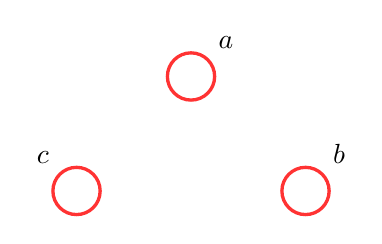
\begin{tikzpicture}[
latentnode/.style={circle, draw=red!80, minimum size=6mm, very thick},
observednode/.style={circle, draw=red!80, fill=cyan!60, minimum size=6mm, very thick},
]

% Defining the nodes
\node[latentnode, label=above right:{$a$}] (a) {};
\node[latentnode, label=above right:{$b$}] (b) [below right=of a] {};
\node[latentnode, label=above left:{$c$}] (c) [below left=of a] {};


% Relationships between latent variables

\end{tikzpicture}
	\caption{Graphical representation of the factorisation $p(a,b,c) = p(a) p(b) p(c)$.}
	\label{fig:bayes-net-1}
\end{figure}

On the contrary, if $\mathcal G = \{\{a,b,c\}, \{\{a, b\}, \{a, c\}, \{b, c\}\}\}$, the joint probability induced by $\mathcal G$ is given by  $p(a,b,c) = p(a)p(b \vert a)p(c \vert a, b)$. The graphical representation of $\mathcal G$ is shown in figure \ref{fig:bayes-net-2}.

\begin{figure}[h!]
	\centering
	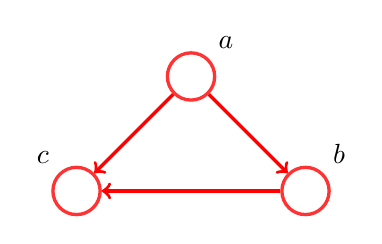
\begin{tikzpicture}[
latentnode/.style={circle, draw=red!80, minimum size=6mm, very thick},
observednode/.style={circle, draw=red!80, fill=cyan!60, minimum size=6mm, very thick},
]

% Defining the nodes
\node[latentnode, label=above right:{$a$}] (a) {};
\node[latentnode, label=above right:{$b$}] (b) [below right=of a] {};
\node[latentnode, label=above left:{$c$}] (c) [below left=of a] {};


% Relationships between latent variables
\draw[->, color=red, very thick] (a) -- (b);
\draw[->, color=red, very thick] (a) -- (c);
\draw[->, color=red, very thick] (b) -- (c);

\end{tikzpicture}
	\caption{Graphical representation of the factorisation $p(a,b,c) = p(a) p(b \vert a) p(c \vert a, b)$.}
	\label{fig:bayes-net-2}
\end{figure}


% then, define the joint distribution over graphical models
More formally, we have the following definition
\begin{definition}
	The joint distribution over a set of random variables $\x = (x_1, \ldots, x_K)$ induced by a Bayesian network is given by the product over each node in the graph conditioned on the variables corresponding to the parents of that node in the graph.
	\begin{equation}
		p({\bf x}) = \prod_{k=1}^K p(x_k \vert \text{Pa}_k).
	\end{equation}
	Where $\text{Pa}_k$ is the set of nodes that directly influence $x_k$.
\end{definition}

It is important to remark that the Bayesian networks considered in this work cannot be strongly connected, i.e., it cannot exist a closed loop in the graph. In that sense, any Bayesian network can be represented as a Directed Acyclic Graph (DAG).

% Then, talk about the use of latent variables and the representation in a bayesian network
% * Use the pLDS as an example to write the complete-data likelihood, and
% * Write it as a probabilistic graphical model
Given any Bayesian network, it is of interest to ask how does the factorisation in a graph changes if a set of random variables are conditioned on another nonintersecting set of random variables. Conditional probabilities allow us to find simpler simpler representations of conditional probabilities which simplifies the model and results in simpler computations. For this, we have the following definition


% Then, write about conditional independence and why it is useful: to simplify the structure of a model and reduce the amount of computations required to perform learning and inference
\begin{definition}
	\textbf{Conditional independence}: Two random variables $a$ and $b$ are said to be conditionally independent over a third random variable $c$, denoted as $a \perp b \vert c$, if the following holds true
	\begin{equation}
		a \perp b \vert c \iff p(a, b \vert c) = p(a \vert c) p(b \vert c).
	\end{equation}
	Equivalently,
	\begin{equation}
		a \perp b \vert c \iff p(a \vert b, c) = p(a \vert c) \text{, } p(b \vert c) = 1.
	\end{equation}
\end{definition}

Given a Bayesian network, we will graphically denote observed random variables as nodes filled in blue. 

\begin{figure}[h!]
	\centering
	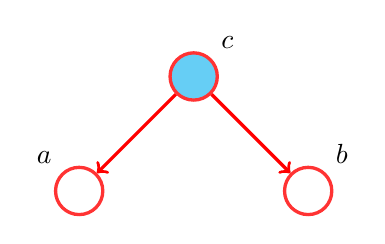
\begin{tikzpicture}[
latentnode/.style={circle, draw=red!80, minimum size=6mm, very thick},
observednode/.style={circle, draw=red!80, fill=cyan!60, minimum size=6mm, very thick},
]

% Defining the nodes
\node[observednode, label=above right:{$c$}] (a) {};
\node[latentnode, label=above right:{$b$}] (b) [below right=of a] {};
\node[latentnode, label=above left:{$a$}] (c) [below left=of a] {};


% Relationships between latent variables
\draw[->, color=red, very thick] (a) -- (b);
\draw[->, color=red, very thick] (a) -- (c);

\end{tikzpicture}
	\caption{Graphical representation of the conditional probabilty $p(a, b\vert c) = p(a \vert c) p(b \vert c)$.}
	\label{fig:bayes-net-3}
\end{figure}


% Next, write about d-separation: determine conditional independence properties directly from the bayes' net
% * Write the d-separation as a theorem (and a reference to a proof)
The distinction between observed and unobserved nodes in a network allows us to specify more complex probabilistic models that have \textit{observed} and \textit{latent} variables. For example, using a Bayesian network, we can write the relationship between variables in a pLDS as presented in figure \ref{fig:lds-gm}.

\begin{figure}[h!]
	\centering
	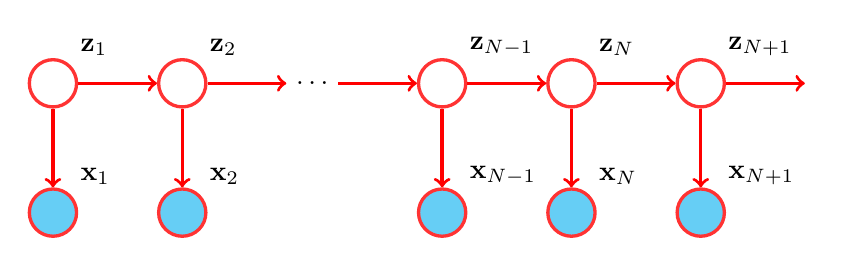
\begin{tikzpicture}[
latentnode/.style={circle, draw=red!80, minimum size=6mm, very thick},
observednode/.style={circle, draw=red!80, fill=cyan!60, minimum size=6mm, very thick},
]

% Defining the nodes
\node[latentnode, label=above right:{${\bf z}_1$}] (z1) {};
\node[latentnode, label=above right:{${\bf z}_2$}] (z2) [right=of z1] {};
\node (transition) [right=of z2] {$\ldots$};
\node[latentnode, label=above right:{${\bf z}_{N-1}$}] (z_nm1) [right=of transition] {};
\node[latentnode, label=above right:{${\bf z}_{N}$}] (zn) [right=of z_nm1] {};
\node[latentnode, label=above right:{${\bf z}_{N+1}$}] (z_np1) [right=of zn] {};
\node (final) [right=of z_np1] {};

% Defining observed nodes
\node[observednode, label=above right:{${\bf x}_1$}] (x1) [below=of z1]{};
\node[observednode, label=above right:{${\bf x}_2$}] (x2) [below=of z2]{};
\node[observednode, label=above right:{${\bf x}_{N-1}$}] (x_nm1) [below=of z_nm1]{};
\node[observednode, label=above right:{${\bf x}_{N}$}] (xn) [below=of zn]{};
\node[observednode, label=above right:{${\bf x}_{N+1}$}] (x_np1) [below=of z_np1]{};


% Relationships between latent variables
\draw[->, color=red, very thick] (z1) -- (z2);
\draw[->, color=red, very thick] (z2) -- (transition);
\draw[->, color=red, very thick] (transition) -- (z_nm1);
\draw[->, color=red, very thick] (z_nm1) -- (zn);
\draw[->, color=red, very thick] (zn) -- (z_np1);
% final node
\draw[->, color=red, very thick] (z_np1) -- (final);

% Relationships between observed and latent variables
\draw[->, color=red, very thick] (z1) -- (x1);
\draw[->, color=red, very thick] (z2) -- (x2);
\draw[->, color=red, very thick] (z_nm1) -- (x_nm1);
\draw[->, color=red, very thick] (zn) -- (xn);
\draw[->, color=red, very thick] (z_np1) -- (x_np1);

\end{tikzpicture}
	\caption{Graphical representation of a pLDS. The filled nodes represent observed variables, whereas the empty nodes represent latent variables.7}
	\label{fig:lds-gm}
\end{figure}

The graphical representation of the Bayesian network induces the following joint distribution between latent and random variables.
\begin{equation}
	p({\bf X}, {\bf Z} \vert\boldsymbol\theta) = p(\z_1)\prod_{n=2}^N p(\z_n\vert \z_{n-1})\prod_{n=1}^N p(\x_n\vert \z_n).
\end{equation}

The graphical representation of a model not only presents an illustration of the relationship between random variables, but it's also used to simplify the representation of conditional probabilities using a set of rules known as \textit{d-separation}. Before we introduce the rules of $d$-separation, we will define what a descendant is, and the types of connections of three nodes in a Bayesian network.

\begin{definition}
	$\mathcal G = \{\mathscr{N}, \mathscr{E}\}$ be a Bayesian network, and let $a \in \mathscr{N}$, $b \in \mathscr{N}$. We define a node $b$ as a \textbf{descendant} of node $a$ if there exists a path from $a$ to $b$.
\end{definition}

Let $a$, $b$, and $c$ be three nodes of a bayesian network $\mathcal G$. We say that
\begin{itemize}
	\item $a$ and $b$ meet head-to-head at $c$ if $a \rightarrow c \leftarrow b $;
	\item $a$ and $b$ meet tail-to-tail at $c$ if $a \leftarrow c \rightarrow b $;
	\item $a$ and $b$ meet head-to-tail at $c$ if $a \rightarrow c \rightarrow b $;
\end{itemize}

\begin{proposition}
	(\textbf{d-separation}) Let $\mathcal G = \{\{A, B, C\}, \mathscr{E}\}$ be a Bayesian network with with $A$, $B$, and $C$ arbitrary nonintersecting set of nodes. To assert whether $A \perp B \vert C$ is induced by the network, we consider all possible paths from any node in $A$ to any node in $B$. Any such path is said to be \textbf{blocked} if it includes a node such that either
	\begin{enumerate}
		\item The arrows on the path meet either head-to-tail or tail-to-tail at a node in the set $C$, or
		\item the arrows meet head-to-head at a node not in the set $C$, or any of its descendants.
	\end{enumerate}
	If all paths are blocked, then $A$ is said to be $d$-separable from $B$ by $C$, and the joint distribution over all variables in the graph satisfy $A \perp B \vert C$.
\end{proposition}

% Finally, 
% * Motivate the following proposition: It helps us decompose the conditional dependencies of the graph and simplify the computations of the E-step
% * Show the following proposition using d-separation

To exemplify the use of $d$-separation, we present the following proposition which will simplify later computations when developing the pLDS model.

\begin{proposition} \label{prop:graphical-models-separation}
	Let $({\bf Z}, {\bf X})$ be the complete-dataset of pLDS model. Then, the following factorisations holds true
	\begin{align}
		p({\bf X}\vert\z_n) &= p({\x_1, \ldots, \x_n \vert \z_n})p({\x_{n+1}, \ldots, \x_N \vert \z_n}), \label{eq:gm-1}\\
		p(\x_1, \ldots, \x_{n-1}\vert \x_n, \z_n) &= p(\x_1, \ldots, \x_{n-1}\vert \z_n), \label{eq:gm-2}\\
		p(\x_1, \ldots, \x_{n-1}\vert \z_{n-1}, \z_{n}) &= p(\x_1, \ldots, \x_{n-1}\vert \z_{n-1}), \label{eq:gm-3}\\
		p(\x_{n+1}, \ldots, \x_N \vert \z_n, \z_{n+1}) &= p(\x_{n+1}, \ldots, \x_N \vert \z_n), \label{eq:gm-4}\\
		p(\x_{n+2}, \ldots, \x_N\vert \x_{n+1}, \z_{n+1}) &= p(\x_{n+2}, \ldots, \x_N \vert \z_{n+1}),\label{eq:gm-5}\\
		p({\bf X}\vert \z_{n-1}, \z_{n}) &= p(\x_1, \ldots, \x_{n-1}\vert \z_{n-1}) \nonumber\\
			&\hspace{1cm}p(\x_n\vert \z_n) p(\x_{n+1}, \ldots, \x_N \vert \z_n), \label{eq:gm-6}\\
		p(\x_{N+1} \vert {\bf X}, \z_{N+1}) &= p(\x_{N+1} \vert \z_{N+1}), \label{eq:gm-7}\\
		p(\z_{N+1} \vert {\bf X}, \z_{N}) &= p(\z_{N+1} \vert \z_{N}). \label{eq:gm-8}\\
	\end{align}
\end{proposition}

\begin{proof}
	All equations in proposition above can be explicitly shown by expanding its components and using the probability rules of sum and product. In this work, we take a visual approach and show that the factorisations hold true using $d$-separation.
	
	Assuming that none of the data in the complete-dataset is observed, the structure of the pLDS is presented in figure \ref{fig:lds-skeleton}.
	
	\begin{figure}[h!]
		\centering
		\resizebox{\columnwidth}{!}{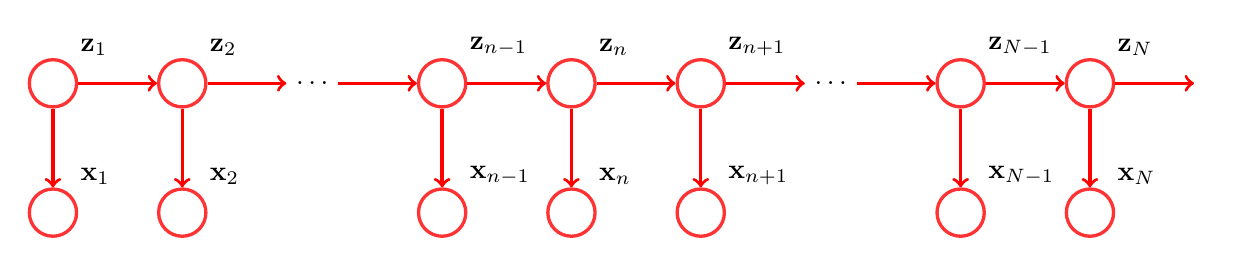
\begin{tikzpicture}[
latentnode/.style={circle, draw=red!80, minimum size=6mm, very thick},
observednode/.style={circle, draw=red!80, minimum size=6mm, very thick},
]

% Defining the nodes
\node[latentnode, label=above right:{${\bf z}_1$}] (z1) {};
\node[latentnode, label=above right:{${\bf z}_2$}] (z2) [right=of z1] {};
\node (transition) [right=of z2] {$\ldots$};
\node[latentnode, label=above right:{${\bf z}_{n-1}$}] (z_nm1) [right=of transition] {};
\node[latentnode, label=above right:{${\bf z}_{n}$}] (zn) [right=of z_nm1] {};
\node[latentnode, label=above right:{${\bf z}_{n+1}$}] (z_np1) [right=of zn] {};
\node (transition2) [right=of z_np1] {$\ldots$};
\node[latentnode, label=above right:{${\bf z}_{N-1}$}] (z_Nm1) [right=of transition2] {};
\node[latentnode, label=above right:{${\bf z}_{N}$}] (zN) [right=of z_Nm1] {};
\node (final) [right=of zN] {};

% Defining observed nodes
\node[observednode, label=above right:{${\bf x}_1$}] (x1) [below=of z1]{};
\node[observednode, label=above right:{${\bf x}_2$}] (x2) [below=of z2]{};
\node[observednode, label=above right:{${\bf x}_{n-1}$}] (x_nm1) [below=of z_nm1]{};
\node[observednode, label=above right:{${\bf x}_{n}$}] (xn) [below=of zn]{};
\node[observednode, label=above right:{${\bf x}_{n+1}$}] (x_np1) [below=of z_np1]{};
\node[observednode, label=above right:{${\bf x}_{N-1}$}] (x_Nm1) [below=of z_Nm1]{};
\node[observednode, label=above right:{${\bf x}_{N}$}] (xN) [below=of zN]{};


% Relationships between latent variables
\draw[->, color=red, very thick] (z1) -- (z2);
\draw[->, color=red, very thick] (z2) -- (transition);
\draw[->, color=red, very thick] (transition) -- (z_nm1);
\draw[->, color=red, very thick] (z_nm1) -- (zn);
\draw[->, color=red, very thick] (zn) -- (z_np1);
\draw[->, color=red, very thick] (z_np1) -- (transition2);
\draw[->, color=red, very thick] (transition2) -- (z_Nm1);
\draw[->, color=red, very thick] (z_Nm1) -- (zN);
\draw[->, color=red, very thick] (zN) -- (final);


% Relationships between observed and latent variables
\draw[->, color=red, very thick] (z1) -- (x1);
\draw[->, color=red, very thick] (z2) -- (x2);
\draw[->, color=red, very thick] (z_nm1) -- (x_nm1);
\draw[->, color=red, very thick] (zn) -- (xn);
\draw[->, color=red, very thick] (z_np1) -- (x_np1);
\draw[->, color=red, very thick] (z_Nm1) -- (x_Nm1);
\draw[->, color=red, very thick] (zN) -- (xN);

\end{tikzpicture}}
		\caption{probabilistic structure of a pLDS.}
		\label{fig:lds-skeleton}
	\end{figure}

	We begin showing equation \eqref{eq:gm-1}. The graph that induces the conditional probability $p(\X \vert \z_n)$ is given by figure \ref{fig:gm-1}. Let $A = \{\x_1, \ldots, \x_{n-1}\}$, $B = \{x_{n+1}, \ldots, \x_N\}$, and $C = \{\z_n\}$. Notice that the connection from any node in $A$ to any node in $B$ meets head-to-tail with $C$. Hence, $A \perp B \vert C$.
	
	\begin{figure}[h!]
		\centering
		\resizebox{\columnwidth}{!}{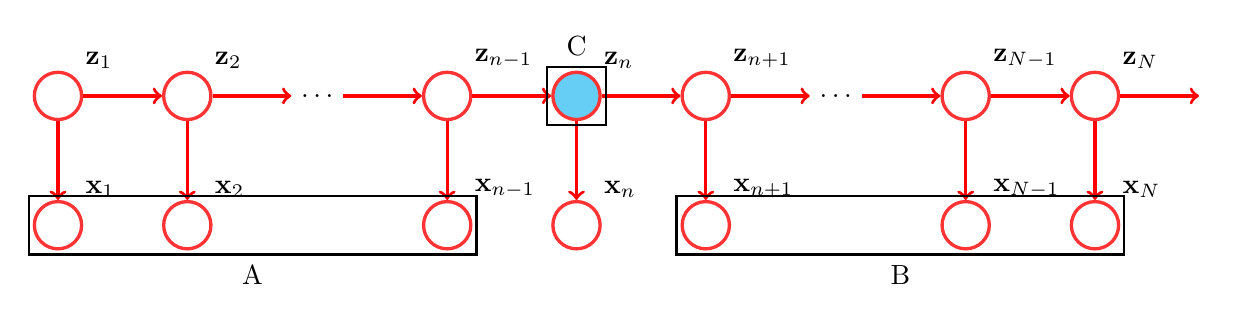
\begin{tikzpicture}[
latentnode/.style={circle, draw=red!80, minimum size=6mm, very thick},
observednode/.style={circle, draw=red!80, fill=cyan!60, minimum size=6mm, very thick},
]

% Defining the nodes
\node[latentnode, label=above right:{${\bf z}_1$}] (z1) {};
\node[latentnode, label=above right:{${\bf z}_2$}] (z2) [right=of z1] {};
\node (transition) [right=of z2] {$\ldots$};
\node[latentnode, label=above right:{${\bf z}_{n-1}$}] (z_nm1) [right=of transition] {};
\node[observednode, label=above right:{${\bf z}_{n}$}] (zn) [right=of z_nm1] {};
\node[latentnode, label=above right:{${\bf z}_{n+1}$}] (z_np1) [right=of zn] {};
\node (transition2) [right=of z_np1] {$\ldots$};
\node[latentnode, label=above right:{${\bf z}_{N-1}$}] (z_Nm1) [right=of transition2] {};
\node[latentnode, label=above right:{${\bf z}_{N}$}] (zN) [right=of z_Nm1] {};
\node (final) [right=of zN] {};

% Defining observed nodes
\node[latentnode, label=above right:{${\bf x}_1$}] (x1) [below=of z1]{};
\node[latentnode, label=above right:{${\bf x}_2$}] (x2) [below=of z2]{};
\node[latentnode, label=above right:{${\bf x}_{n-1}$}] (x_nm1) [below=of z_nm1]{};
\node[latentnode, label=above right:{${\bf x}_{n}$}] (xn) [below=of zn]{};
\node[latentnode, label=above right:{${\bf x}_{n+1}$}] (x_np1) [below=of z_np1]{};
\node[latentnode, label=above right:{${\bf x}_{N-1}$}] (x_Nm1) [below=of z_Nm1]{};
\node[latentnode, label=above right:{${\bf x}_{N}$}] (xN) [below=of zN]{};


% Relationships between latent variables
\draw[->, color=red, very thick] (z1) -- (z2);
\draw[->, color=red, very thick] (z2) -- (transition);
\draw[->, color=red, very thick] (transition) -- (z_nm1);
\draw[->, color=red, very thick] (z_nm1) -- (zn);
\draw[->, color=red, very thick] (zn) -- (z_np1);
\draw[->, color=red, very thick] (z_np1) -- (transition2);
\draw[->, color=red, very thick] (transition2) -- (z_Nm1);
\draw[->, color=red, very thick] (z_Nm1) -- (zN);
\draw[->, color=red, very thick] (zN) -- (final);


% Relationships between observed and latent variables
\draw[->, color=red, very thick] (z1) -- (x1);
\draw[->, color=red, very thick] (z2) -- (x2);
\draw[->, color=red, very thick] (z_nm1) -- (x_nm1);
\draw[->, color=red, very thick] (zn) -- (xn);
\draw[->, color=red, very thick] (z_np1) -- (x_np1);
\draw[->, color=red, very thick] (z_Nm1) -- (x_Nm1);
\draw[->, color=red, very thick] (zN) -- (xN);

\node[draw, thick, inner sep=0.5mm,label=below:A,fit=(x1) (x_nm1)] {};
\node[draw, thick, inner sep=0.5mm,label=below:B,fit=(x_np1) (xN)] {};
\node[draw, thick, inner sep=0.5mm,label=above:C,fit=(zn)] {};

\end{tikzpicture}}
		\caption{gm1.}
		\label{fig:gm-1}
	\end{figure}
	
	Next, we show equation \eqref{eq:gm-2}. Taking $A = \{\x_1, \ldots, \x_{n-1}\}$, $B = \{\x_n\}$, and $C = \{\z_n\}$, we observe that any node in $A$ to $\x_n$ meet head-to-tail at $\z_n$. Hence $A \perp \x_n \vert \z_n$.
	\begin{figure}[h!]
		\centering
		\resizebox{\columnwidth}{!}{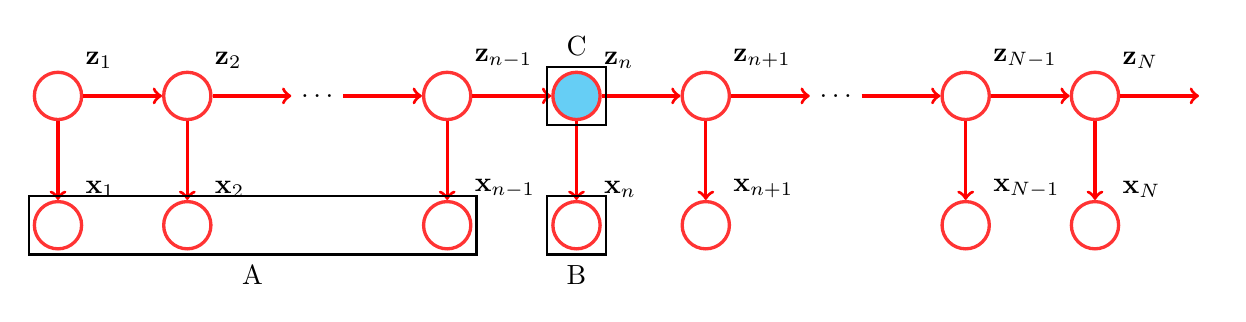
\begin{tikzpicture}[
latentnode/.style={circle, draw=red!80, minimum size=6mm, very thick},
observednode/.style={circle, draw=red!80, fill=cyan!60, minimum size=6mm, very thick},
]

% Defining the nodes
\node[latentnode, label=above right:{${\bf z}_1$}] (z1) {};
\node[latentnode, label=above right:{${\bf z}_2$}] (z2) [right=of z1] {};
\node (transition) [right=of z2] {$\ldots$};
\node[latentnode, label=above right:{${\bf z}_{n-1}$}] (z_nm1) [right=of transition] {};
\node[observednode, label=above right:{${\bf z}_{n}$}] (zn) [right=of z_nm1] {};
\node[latentnode, label=above right:{${\bf z}_{n+1}$}] (z_np1) [right=of zn] {};
\node (transition2) [right=of z_np1] {$\ldots$};
\node[latentnode, label=above right:{${\bf z}_{N-1}$}] (z_Nm1) [right=of transition2] {};
\node[latentnode, label=above right:{${\bf z}_{N}$}] (zN) [right=of z_Nm1] {};
\node (final) [right=of zN] {};

% Defining observed nodes
\node[latentnode, label=above right:{${\bf x}_1$}] (x1) [below=of z1]{};
\node[latentnode, label=above right:{${\bf x}_2$}] (x2) [below=of z2]{};
\node[latentnode, label=above right:{${\bf x}_{n-1}$}] (x_nm1) [below=of z_nm1]{};
\node[latentnode, label=above right:{${\bf x}_{n}$}] (xn) [below=of zn]{};
\node[latentnode, label=above right:{${\bf x}_{n+1}$}] (x_np1) [below=of z_np1]{};
\node[latentnode, label=above right:{${\bf x}_{N-1}$}] (x_Nm1) [below=of z_Nm1]{};
\node[latentnode, label=above right:{${\bf x}_{N}$}] (xN) [below=of zN]{};


% Relationships between latent variables
\draw[->, color=red, very thick] (z1) -- (z2);
\draw[->, color=red, very thick] (z2) -- (transition);
\draw[->, color=red, very thick] (transition) -- (z_nm1);
\draw[->, color=red, very thick] (z_nm1) -- (zn);
\draw[->, color=red, very thick] (zn) -- (z_np1);
\draw[->, color=red, very thick] (z_np1) -- (transition2);
\draw[->, color=red, very thick] (transition2) -- (z_Nm1);
\draw[->, color=red, very thick] (z_Nm1) -- (zN);
\draw[->, color=red, very thick] (zN) -- (final);


% Relationships between observed and latent variables
\draw[->, color=red, very thick] (z1) -- (x1);
\draw[->, color=red, very thick] (z2) -- (x2);
\draw[->, color=red, very thick] (z_nm1) -- (x_nm1);
\draw[->, color=red, very thick] (zn) -- (xn);
\draw[->, color=red, very thick] (z_np1) -- (x_np1);
\draw[->, color=red, very thick] (z_Nm1) -- (x_Nm1);
\draw[->, color=red, very thick] (zN) -- (xN);

\node[draw, thick, inner sep=0.5mm,label=below:A,fit=(x1) (x_nm1)] {};
\node[draw, thick, inner sep=0.5mm,label=below:B,fit=(xn)] {};
\node[draw, thick, inner sep=0.5mm,label=above:C,fit=(zn)] {};

\end{tikzpicture}}
		\caption{gm2.}
		\label{fig:gm-2}
	\end{figure}

	Following the same logic, we can show that equations \eqref{eq:gm-3}, \eqref{eq:gm-4}, \eqref{eq:gm-5}, \eqref{eq:gm-7}, and \eqref{eq:gm-8}  meet either head-to-tail or tail-to-tail at a node in the set $C$. We present the graphical representations of equations \eqref{eq:gm-3}, \eqref{eq:gm-4}, and \eqref{eq:gm-5} in figures \ref{fig:gm-3}, \ref{fig:gm-4}, and \ref{fig:gm-5}.
	\begin{figure}[h!]
		\centering
		\resizebox{\columnwidth}{!}{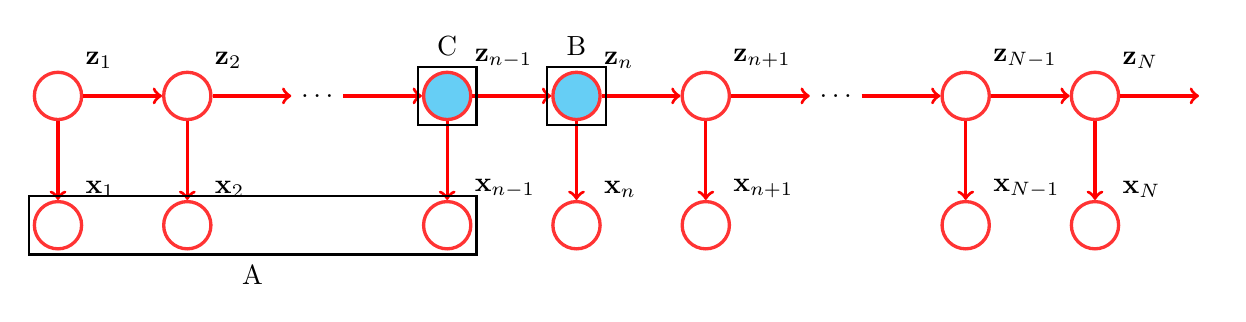
\begin{tikzpicture}[
latentnode/.style={circle, draw=red!80, minimum size=6mm, very thick},
observednode/.style={circle, draw=red!80, fill=cyan!60, minimum size=6mm, very thick},
]

% Defining the nodes
\node[latentnode, label=above right:{${\bf z}_1$}] (z1) {};
\node[latentnode, label=above right:{${\bf z}_2$}] (z2) [right=of z1] {};
\node (transition) [right=of z2] {$\ldots$};
\node[observednode, label=above right:{${\bf z}_{n-1}$}] (z_nm1) [right=of transition] {};
\node[observednode, label=above right:{${\bf z}_{n}$}] (zn) [right=of z_nm1] {};
\node[latentnode, label=above right:{${\bf z}_{n+1}$}] (z_np1) [right=of zn] {};
\node (transition2) [right=of z_np1] {$\ldots$};
\node[latentnode, label=above right:{${\bf z}_{N-1}$}] (z_Nm1) [right=of transition2] {};
\node[latentnode, label=above right:{${\bf z}_{N}$}] (zN) [right=of z_Nm1] {};
\node (final) [right=of zN] {};

% Defining observed nodes
\node[latentnode, label=above right:{${\bf x}_1$}] (x1) [below=of z1]{};
\node[latentnode, label=above right:{${\bf x}_2$}] (x2) [below=of z2]{};
\node[latentnode, label=above right:{${\bf x}_{n-1}$}] (x_nm1) [below=of z_nm1]{};
\node[latentnode, label=above right:{${\bf x}_{n}$}] (xn) [below=of zn]{};
\node[latentnode, label=above right:{${\bf x}_{n+1}$}] (x_np1) [below=of z_np1]{};
\node[latentnode, label=above right:{${\bf x}_{N-1}$}] (x_Nm1) [below=of z_Nm1]{};
\node[latentnode, label=above right:{${\bf x}_{N}$}] (xN) [below=of zN]{};


% Relationships between latent variables
\draw[->, color=red, very thick] (z1) -- (z2);
\draw[->, color=red, very thick] (z2) -- (transition);
\draw[->, color=red, very thick] (transition) -- (z_nm1);
\draw[->, color=red, very thick] (z_nm1) -- (zn);
\draw[->, color=red, very thick] (zn) -- (z_np1);
\draw[->, color=red, very thick] (z_np1) -- (transition2);
\draw[->, color=red, very thick] (transition2) -- (z_Nm1);
\draw[->, color=red, very thick] (z_Nm1) -- (zN);
\draw[->, color=red, very thick] (zN) -- (final);


% Relationships between observed and latent variables
\draw[->, color=red, very thick] (z1) -- (x1);
\draw[->, color=red, very thick] (z2) -- (x2);
\draw[->, color=red, very thick] (z_nm1) -- (x_nm1);
\draw[->, color=red, very thick] (zn) -- (xn);
\draw[->, color=red, very thick] (z_np1) -- (x_np1);
\draw[->, color=red, very thick] (z_Nm1) -- (x_Nm1);
\draw[->, color=red, very thick] (zN) -- (xN);

\node[draw, thick, inner sep=0.5mm,label=below:A,fit=(x1) (x_nm1)] {};
\node[draw, thick, inner sep=0.5mm,label=above:B,fit=(zn)] {};
\node[draw, thick, inner sep=0.5mm,label=above:C,fit=(z_nm1)] {};

\end{tikzpicture}}
		\caption{gm3.}
		\label{fig:gm-3}
	\end{figure}
	
	\begin{figure}[h!]
		\centering
		\resizebox{\columnwidth}{!}{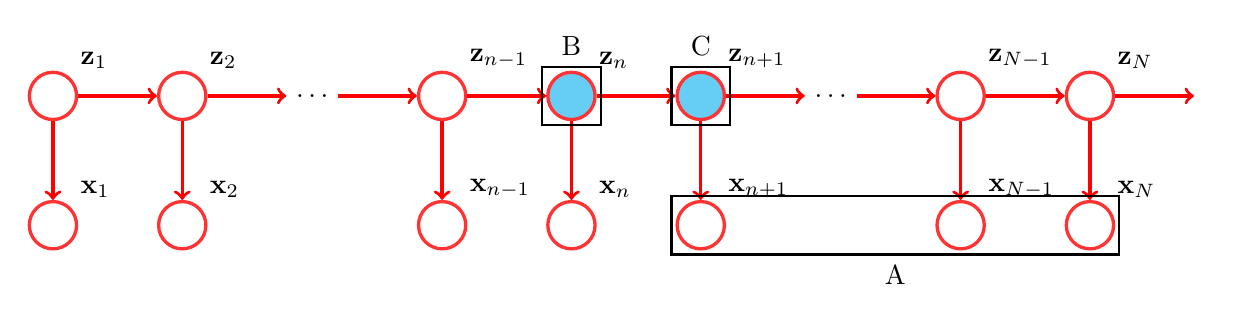
\begin{tikzpicture}[
latentnode/.style={circle, draw=red!80, minimum size=6mm, very thick},
observednode/.style={circle, draw=red!80, fill=cyan!60, minimum size=6mm, very thick},
]

% Defining the nodes
\node[latentnode, label=above right:{${\bf z}_1$}] (z1) {};
\node[latentnode, label=above right:{${\bf z}_2$}] (z2) [right=of z1] {};
\node (transition) [right=of z2] {$\ldots$};
\node[latentnode, label=above right:{${\bf z}_{n-1}$}] (z_nm1) [right=of transition] {};
\node[observednode, label=above right:{${\bf z}_{n}$}] (zn) [right=of z_nm1] {};
\node[observednode, label=above right:{${\bf z}_{n+1}$}] (z_np1) [right=of zn] {};
\node (transition2) [right=of z_np1] {$\ldots$};
\node[latentnode, label=above right:{${\bf z}_{N-1}$}] (z_Nm1) [right=of transition2] {};
\node[latentnode, label=above right:{${\bf z}_{N}$}] (zN) [right=of z_Nm1] {};
\node (final) [right=of zN] {};

% Defining observed nodes
\node[latentnode, label=above right:{${\bf x}_1$}] (x1) [below=of z1]{};
\node[latentnode, label=above right:{${\bf x}_2$}] (x2) [below=of z2]{};
\node[latentnode, label=above right:{${\bf x}_{n-1}$}] (x_nm1) [below=of z_nm1]{};
\node[latentnode, label=above right:{${\bf x}_{n}$}] (xn) [below=of zn]{};
\node[latentnode, label=above right:{${\bf x}_{n+1}$}] (x_np1) [below=of z_np1]{};
\node[latentnode, label=above right:{${\bf x}_{N-1}$}] (x_Nm1) [below=of z_Nm1]{};
\node[latentnode, label=above right:{${\bf x}_{N}$}] (xN) [below=of zN]{};


% Relationships between latent variables
\draw[->, color=red, very thick] (z1) -- (z2);
\draw[->, color=red, very thick] (z2) -- (transition);
\draw[->, color=red, very thick] (transition) -- (z_nm1);
\draw[->, color=red, very thick] (z_nm1) -- (zn);
\draw[->, color=red, very thick] (zn) -- (z_np1);
\draw[->, color=red, very thick] (z_np1) -- (transition2);
\draw[->, color=red, very thick] (transition2) -- (z_Nm1);
\draw[->, color=red, very thick] (z_Nm1) -- (zN);
\draw[->, color=red, very thick] (zN) -- (final);


% Relationships between observed and latent variables
\draw[->, color=red, very thick] (z1) -- (x1);
\draw[->, color=red, very thick] (z2) -- (x2);
\draw[->, color=red, very thick] (z_nm1) -- (x_nm1);
\draw[->, color=red, very thick] (zn) -- (xn);
\draw[->, color=red, very thick] (z_np1) -- (x_np1);
\draw[->, color=red, very thick] (z_Nm1) -- (x_Nm1);
\draw[->, color=red, very thick] (zN) -- (xN);

\node[draw, thick, inner sep=0.5mm,label=below:A,fit=(x_np1) (xN)] {};
\node[draw, thick, inner sep=0.5mm,label=above:B,fit=(zn)] {};
\node[draw, thick, inner sep=0.5mm,label=above:C,fit=(z_np1)] {};

\end{tikzpicture}}
		\caption{gm4.}
		\label{fig:gm-4}
	\end{figure}
	
	\begin{figure}[h!]
		\centering
		\resizebox{\columnwidth}{!}{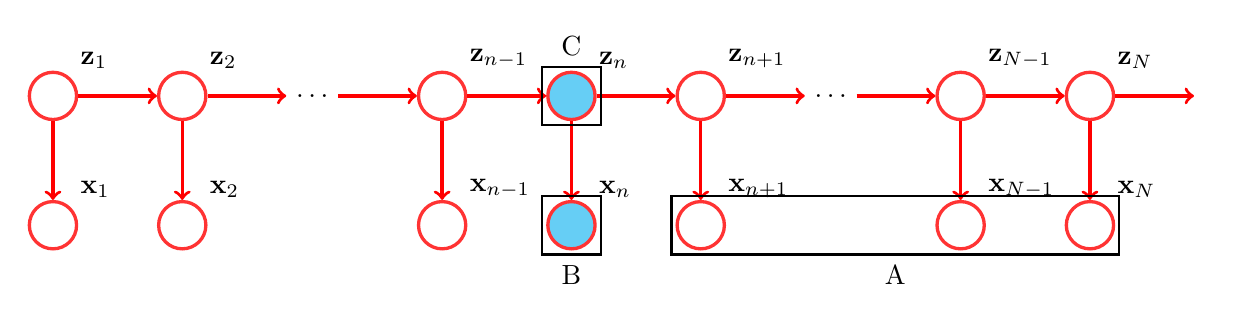
\begin{tikzpicture}[
latentnode/.style={circle, draw=red!80, minimum size=6mm, very thick},
observednode/.style={circle, draw=red!80, fill=cyan!60, minimum size=6mm, very thick},
]

% Defining the nodes
\node[latentnode, label=above right:{${\bf z}_1$}] (z1) {};
\node[latentnode, label=above right:{${\bf z}_2$}] (z2) [right=of z1] {};
\node (transition) [right=of z2] {$\ldots$};
\node[latentnode, label=above right:{${\bf z}_{n-1}$}] (z_nm1) [right=of transition] {};
\node[observednode, label=above right:{${\bf z}_{n}$}] (zn) [right=of z_nm1] {};
\node[latentnode, label=above right:{${\bf z}_{n+1}$}] (z_np1) [right=of zn] {};
\node (transition2) [right=of z_np1] {$\ldots$};
\node[latentnode, label=above right:{${\bf z}_{N-1}$}] (z_Nm1) [right=of transition2] {};
\node[latentnode, label=above right:{${\bf z}_{N}$}] (zN) [right=of z_Nm1] {};
\node (final) [right=of zN] {};

% Defining observed nodes
\node[latentnode, label=above right:{${\bf x}_1$}] (x1) [below=of z1]{};
\node[latentnode, label=above right:{${\bf x}_2$}] (x2) [below=of z2]{};
\node[latentnode, label=above right:{${\bf x}_{n-1}$}] (x_nm1) [below=of z_nm1]{};
\node[observednode, label=above right:{${\bf x}_{n}$}] (xn) [below=of zn]{};
\node[latentnode, label=above right:{${\bf x}_{n+1}$}] (x_np1) [below=of z_np1]{};
\node[latentnode, label=above right:{${\bf x}_{N-1}$}] (x_Nm1) [below=of z_Nm1]{};
\node[latentnode, label=above right:{${\bf x}_{N}$}] (xN) [below=of zN]{};


% Relationships between latent variables
\draw[->, color=red, very thick] (z1) -- (z2);
\draw[->, color=red, very thick] (z2) -- (transition);
\draw[->, color=red, very thick] (transition) -- (z_nm1);
\draw[->, color=red, very thick] (z_nm1) -- (zn);
\draw[->, color=red, very thick] (zn) -- (z_np1);
\draw[->, color=red, very thick] (z_np1) -- (transition2);
\draw[->, color=red, very thick] (transition2) -- (z_Nm1);
\draw[->, color=red, very thick] (z_Nm1) -- (zN);
\draw[->, color=red, very thick] (zN) -- (final);


% Relationships between observed and latent variables
\draw[->, color=red, very thick] (z1) -- (x1);
\draw[->, color=red, very thick] (z2) -- (x2);
\draw[->, color=red, very thick] (z_nm1) -- (x_nm1);
\draw[->, color=red, very thick] (zn) -- (xn);
\draw[->, color=red, very thick] (z_np1) -- (x_np1);
\draw[->, color=red, very thick] (z_Nm1) -- (x_Nm1);
\draw[->, color=red, very thick] (zN) -- (xN);

\node[draw, thick, inner sep=0.5mm,label=below:A,fit=(x_np1) (xN)] {};
\node[draw, thick, inner sep=0.5mm,label=below:B,fit=(xn)] {};
\node[draw, thick, inner sep=0.5mm,label=above:C,fit=(zn)] {};

\end{tikzpicture}}
		\caption{gm5.}
		\label{fig:gm-5}
	\end{figure}
	
	To show equation \eqref{eq:gm-6}, consider
	\begin{align}
		p(\X \vert \z_{n-1}, \z_n) &= p(\x_1, \ldots, \x_N \vert \z_{n-1},\z_n)\\
		 &= p(\x_n \vert \z_{n-1}, \z_n) p(\x_1, \ldots, \x_{n-1}, \x_{n+1}, \ldots, \x_N \vert \x_n, \z_{n-1}, \z_n)\\
		&= p(\x_n \vert \z_{n-1}, \z_n) p(\x_1, \ldots, \x_{n-1} \vert \x_n, \z_{n-1}, \z_n) \nonumber\\
			&\hspace{1cm} p(\x_{n+1}, \ldots, \x_N \vert \x_1, \ldots, \x_N, \z_{n-1}, \z_n). \label{eq:part-gm-6}
	\end{align}
	
	Using equation \eqref{eq:gm-2} we have $p(\x_n \vert \z_{n-1}, \z_n) = p(\x_n \vert \z_n)$. Furthermore, using equations \eqref{eq:gm-2} and \eqref{eq:gm-3}, $p(\x_1, \ldots, \x_{n-1} \vert \x_n, \z_{n-1}, \z_n) = p(\x_1, \ldots, \x_{n-1} \vert \z_{n-1})$. Finally, from equations \eqref{eq:gm-4}, and \eqref{eq:gm-5} we obtain  $p(\x_{n+1}, \ldots, \x_N \vert \x_1, \ldots, \x_N, \z_{n-1}, \z_n) = p(\x_{n+1}, \ldots, \x_N \vert  \z_{n})$. Using these results and plugging the values in \eqref{eq:part-gm-6} yields equation \eqref{eq:gm-6}.
\end{proof}


\subsection{The EM algorithm}

As we have previously mentioned, in order to find the parameters $\boldsymbol{\theta}$ that best represent the complete-dataset, we require to maximise the log-likelihood of the complete dataset with respect to each of the parameters in $\boldsymbol{\theta}$. In this section, we present the Expectation Maximisation (EM) algorithm: a two-step iterative approach that maximises the log-likelihood of the complete-dataset. Broadly speaking, the EM algorithm is divided into two steps: the E-step attempts to estimate a plausible dataset $\Z$ given current estimates of $\boldsymbol\theta$; the M-step, fixes the estimated values of $\Z$ and updates $\boldsymbol{\theta}$. Under certain conditions, it can be shown that the EM algorithm converges to a local maximum (\cite{pml1Book}). We formally derive the EM algorithm in the following three propositions.

\begin{proposition} \label{prop:log-likelihood-partition}
	The log-likelihood $\log p({\bf X} \vert \boldsymbol{\theta})$ can be written as the sum of two factors
	\begin{equation}
		\log p({\bf X} \vert \boldsymbol{\theta}) = \mathcal{L}(q, \boldsymbol{\theta}) +\KL{q}{p}.
	\end{equation}
	Where
	\begin{align}
		\mathcal{L}(q, \boldsymbol{\theta}) &= \int q({\bf Z})\log\left(\frac{p({\bf X}, {\bf Z} \vert \boldsymbol\theta)}{q({\bf Z})}\right) d{\bf Z},\\
		\text{KL}(q \vert\vert p) &= \int q({\bf Z}) \log\left(\frac{q({\bf Z})}{p({\bf Z}\vert {\bf X}, \boldsymbol\theta)}\right) d{\bf Z}.
	\end{align}
\end{proposition}

\begin{proof}
	The proof follows directly from the sum of the terms $\mathcal{L}(q, \boldsymbol{\theta})$, and  $\text{KL}(q \vert\vert p)$:
	\begin{align}
		\mathcal{L}(q, \boldsymbol{\theta}) + \KL{q}{p} &= \int q({\bf Z})\log\left(\frac{p({\bf X}, {\bf Z} \vert \boldsymbol\theta)}{q({\bf Z})}\right) d{\bf Z} + \int q({\bf Z}) \log\left(\frac{q({\bf Z})}{p({\bf Z}\vert {\bf X}, \boldsymbol\theta)}\right) d{\bf Z}\\
		&= \int q({\bf Z})\left(\log p({\bf X, {\bf Z} \vert \boldsymbol{\theta}}) - \log q({\bf Z}) + \log q({\bf Z}) - \log p({\bf Z} \vert {\bf X}, \boldsymbol\theta)\right) d{\bf Z}\\
		&= \int q({\bf Z})\left(\log p({\bf X} \vert \boldsymbol{\theta}) + \log p({\bf Z} \vert {\bf X}, \boldsymbol{\theta}) - \log p({\bf Z} \vert {\bf X}, \boldsymbol\theta)\right) d{\bf Z}\\
		&= \log p({\bf X}\vert \boldsymbol\theta).
	\end{align}
\end{proof}

The term $\mathcal{L}(q, \boldsymbol\theta)$ in proposition \ref{prop:log-likelihood-partition} is called the lower bound, and the term $\KL{q}{p}$ is known as the Kullback-Leibler divergence of the distributions $p$ and $q$. 


%TODO: define a set \mathcal Q of "valid" distributions.
%TODO: why is it relevant to only maximise the lower bound L?
\begin{proposition} (\textbf{E-step})
	The function $q({\bf Z})$ that maximises the lower bound $\mathcal L(q, \boldsymbol{\theta}$) is given by
	\begin{equation}
		q(\Z) = \max_{\hat q} \mathcal{L}(\hat q, \boldsymbol\theta) = p({\bf Z} \vert {\bf X}, \boldsymbol\theta).
	\end{equation}
\end{proposition}

\begin{proof}
	We begin by rewriting the lower bound term. We obtain that
	\begin{align}
		\mathcal{L}(q, \boldsymbol\theta) &= \int q(\Z)\log\left(\frac{p(\X, \Z \vert \boldsymbol\theta)}{q(\Z)}\right) d{\bf Z}\\
		&= \int q(\Z) \left(\log p(\X\vert\boldsymbol\theta) + \log\left( \frac{p(\Z \vert \X, \boldsymbol\theta)}{q(\Z)} \right) \right) d\Z\\
		&= \log p(\X \vert \boldsymbol{\theta}) - \int q(\Z) \log\left(\frac{q(\Z)}{p(\Z \vert \X, \boldsymbol\theta)}\right) d\Z\\
		&= \log p(\X \vert \boldsymbol\theta) - \KL{q}{p}. \label{eq:part-L-rewrite}
	\end{align}
	
	To find the function $q$ that maximises \eqref{eq:part-L-rewrite}, we notice that the first term does not depend on $q$. Furthermore, we observe that the second term is the negative Kullback-Leibler divergence between $q$ and $p$. The KL diverge is nonnegative with equality to zero if and only if $q=p$   (for a proof, see \cite{pml1Book}). Therefore, the function $q(\Z)$ that maximises the lower bound is given by $p(\Z \vert \X, \boldsymbol\theta)$.
\end{proof}

\begin{proposition}\label{prop:m-step}
	(\textbf{M-step}) Maximising $\mathcal{L}(q, \boldsymbol{\theta})$ over $\boldsymbol{\theta}$ at fixed $q({\bf Z}) = p({\bf Z} \vert {\bf X}, \boldsymbol\theta^\text{old})$ is equivalent to maximising the function
	\begin{equation}
		Q(\boldsymbol{\theta}, \boldsymbol{\theta}^\text{old}) = \mathbb{E}_{{\bf Z}\vert {\bf X}, \boldsymbol{\theta}^\text{old}}[\log p({\bf X}, {\bf Z}\vert \boldsymbol\theta)]
	\end{equation}
\end{proposition}

\begin{proof}
	We show proposition \ref{prop:m-step} by rewriting the maximisation of the lower bound with fixed $q$. We obtain
	\begin{align}
		\boldsymbol{\theta}^\text{new} &= \argmax{\boldsymbol\theta} \mathcal{L}(q, \boldsymbol\theta)\\
		&= \argmax{\boldsymbol{\theta}} \int p(\Z \vert \X, \boldsymbol{\theta}^\text{old}) \log\left(\frac{p(\X, \Z \vert \boldsymbol\theta)}{p(\Z \vert \X, \boldsymbol\theta^\text{old})}\right) d\Z\\
		&= \argmax{\boldsymbol{\theta}} \int p(\Z \vert \X, \boldsymbol{\theta} ^\text{old}) \log p(\X, \Z \vert \boldsymbol\theta) d\Z - \int p(\Z \vert \X, \boldsymbol{\theta}^\text{old}) \log p(\Z \vert \X, \boldsymbol{\theta}^\text{old})\\
		&= \argmax{\boldsymbol{\theta}} \mathbb{E}_{{\bf Z}\vert {\bf X}, \boldsymbol{\theta}^\text{old}}[\log p({\bf X}, {\bf Z}\vert \boldsymbol\theta)].
	\end{align}
\end{proof}

% TODO: the EM algorithm converges under some conditions which our LDS model
% has. Write

\section{Deriving a model for the pLDS}
In this section, we derive the E-step and the M-steps for the linear dynamical system presented in the previous section.

\subsection{The E-step}
To make use of the E-step, it is helpful to distinguish which elements depend on $\z_n$. Consider

\begin{align}
	\log p({\bf X}, {\bf Z}\vert \boldsymbol\theta) &= \log p(\z_1) + \sum_{n=2}^N \log p(\z_n\vert \z_{n-1}) + \sum_{n=1}^N \log p(\x_n\vert \z_n)\\
	   &=\frac{1}{2}\log\vert{\bf V}_0^{-1}\vert - \frac{1}{2}(\z_1 - \boldsymbol\mu_0)^T{\bf V}_0^{-1}(\z_1 - \boldsymbol\mu_0) \nonumber \\
	   &\hspace{1cm}+ \sum_{n=2}^N \frac{1}{2}\log\vert\boldsymbol\Gamma^{-1}\vert - \frac{1}{2}(\z_n - {\bf A z}_{n-1})^T\boldsymbol{\Gamma}^{-1}(\z_n - {\bf A z}_{n-1}) \nonumber \\
	   &\hspace{1cm}+\sum_{n=1}^N \frac{1}{2}\log\vert\boldsymbol\Sigma\vert -\frac{1}{2}(\x_n - {\bf C z}_n)^T \boldsymbol{\Sigma}^{-1}(\x_n - {\bf C z}_n) + \text{const.}\\
	   &= \frac{1}{2}\log \vert
	  {\bf V}_0^{-1}\vert -\frac{1}{2}\left[\text{Tr}\left(\z_1 \z_1^T {\bf V}_0^{-1}\right) -2 \z_1^T{\bf V}_0^{-1}\boldsymbol\mu_0 + \boldsymbol\mu_0^T {\bf V}_0^{-1}\boldsymbol\mu_0\right] \nonumber \\
	  &\hspace{1cm}+ \frac{N-1}{2}\log\vert\boldsymbol\Gamma^{-1}\vert + \frac{N}{2}\log\vert \boldsymbol\Sigma^{-1}\vert \nonumber \\
	  &\hspace{1cm}-\frac{1}{2} \sum_{n=2}^{N}\text{Tr}\big(\z_n\z_n^T\boldsymbol\Gamma^{-1} -{\bf A} \z_{n-1}\z_n^T\boldsymbol\Gamma^{-1} - \nonumber\\
	  &\hspace{1.8cm}{\bf A}^T\boldsymbol{\Gamma}^{-1}\z_n\z_{n-1}^T + {\bf A}^T \boldsymbol\Gamma^{-1}{\bf A}\z_{n-1}\z_{n-1}^T\big) \nonumber\\
	  &\hspace{1cm}-\frac{1}{2}\sum_{n=1}^N\big[\x_n^T\boldsymbol{\Sigma}^{-1}\x_n - \z_n^T{\bf C}^T\boldsymbol\Sigma^{-1}\x_n - \x_n^T\boldsymbol{\Sigma}^{-1}{\bf C}\z_n  \\
	  &\hspace{1cm} + \text{Tr}(\z_n\z_n^T{\bf C}^T\boldsymbol\Sigma^{-1}{\bf C})\big] + \text{const.} \label{eq:complete-log-likelihood}
\end{align}

Where const. are the terms that do not depend on $\boldsymbol{\theta}$. From equation \eqref{eq:complete-log-likelihood}, we observe that the expectation with respect to the posterior distribution is completely determined by the expectations $\mathbb{E}[\z_n]$, $\mathbb{E}[\z_n\z_{n}^{T}]$, and  $\mathbb{E}[\z_n\z_{n-1}^{T}]$. That is,

\begin{align}
	Q(\boldsymbol\theta, \boldsymbol\theta^\text{old}) &= \frac{1}{2}\log \vert
	  {\bf V}_0^{-1}\vert -\frac{1}{2}\left[\text{Tr}\left(\mathbb{E}\left[\z_1 \z_1^T\right] {\bf V}_0^{-1}\right) -2 \mathbb{E}\left[\z_1\right]^T{\bf V}_0^{-1}\boldsymbol\mu_0 + \boldsymbol\mu_0^T {\bf V}_0^{-1}\boldsymbol\mu_0\right] \nonumber \\
	  &\hspace{1cm}+ \frac{N-1}{2}\log\vert\boldsymbol\Gamma^{-1}\vert + \frac{N}{2}\log\vert \boldsymbol\Sigma^{-1}\vert \nonumber \\
	  &\hspace{1cm}-\frac{1}{2} \sum_{n=2}^{N}\text{Tr}\big(\expectation{\z_n\z_n^T}\boldsymbol\Gamma^{-1} - {\bf A}\expectation{\z_{n-1}\z_n^T}\boldsymbol\Gamma^{-1} \nonumber\\
	  &\hspace{1.8cm} - {\bf A}^T\boldsymbol{\Gamma}^{-1}\expectation{\z_n\z_{n-1}^T} + {\bf A}^T\boldsymbol\Gamma^{-1}{\bf A}\expectation{\z_{n-1}\z_{n-1}^T}\big) \nonumber\\
	  &\hspace{1cm}-\frac{1}{2}\sum_{n=1}^N\big[\x_n^T\boldsymbol{\Sigma}^{-1}\x_n-\expectation{\z_n^T}{\bf C}^T \boldsymbol\Sigma^{-1}\x_n - \x_n^T\boldsymbol\Sigma^{-1}{\bf C}\expectation{\z_n} \nonumber\\
	  &\hspace{1cm} + \text{Tr}(\mathbb{E}\left[\z_n\z_n^T\right]{\bf C}^T\boldsymbol\Sigma^{-1}{\bf C})\big] + \text{const.}  \label{eq:Q-LDS}
\end{align}


To compute the expected values of the latent variables, we first find the posterior distribution of the latent variables $\gamma(\z_n) := p(\z_n\vert {\bf X})$, and $\xi(\z_{n-1}, \z_{n}) := p(\z_{n-1}, \z_n\vert {\bf X})$. As we will see, computing these distributions show that their values are depended on past and future 

%why is it useful?

\begin{proposition}\label{prop:gamma-factorisation}
	The term $\gamma(\z_n)$ can be written as a product of the joint probabilities of the first $n$ observations and $\z_n$, and the conditional probability of the observations that follow $\z_n$ conditional on $\z_n$.
\end{proposition}

\begin{proof}
Denote $\alpha(\z_n) := p(\x_1, \ldots, \x_n, \z_n)$ as the joint probability of the observed data up to $n$, and $\beta(\z_n) := p(\x_{n+1}, \ldots, \x_N\vert \z_n)$ as the probability of all data that follows the $n$-th observation, conditional on the $n$-th latent variable $\z_n$. Next, Consider  $\gamma(\z_n)$ and equation \eqref{eq:gm-1} from proposition \ref{prop:graphical-models-separation}. We have
\begin{align}
	\gamma(\z_n) &= p(\z_n \vert {\bf X})\\
					  &= \frac{1}{p(\x)}p(\z_n)p({\bf X} \vert \z_n)\\
					  &= \frac{1}{p(\x)} p(\z_n) p(\x_1, \ldots, \x_n\vert \z_n) p(\x_{n+1}, \ldots, \x_N\vert \z_n) \label{eq:gamma-part-1}\\
					  &= \frac{1}{p(\x)}p(\x_1, \ldots, \x_n, \z_n) p(\x_{n+1}, \ldots, \x_N\vert \z_n)\\
					  &= \frac{1}{p(\x)}\alpha(\z_n)\beta(\z_n).
\end{align}

Where we have used equation \eqref{eq:gm-1} in proposition \ref{prop:graphical-models-separation} to arrive at equation \eqref{eq:gamma-part-1}.
\end{proof}


% Here we show that the xi can also be written in terms of alpha and beta
\begin{proposition}\label{prop:xi-factorisation}
	The term $\xi(\z_{n-1}, \z_n)$ can be written in terms of $\alpha({\cdot})$, and $\beta(\cdot)$
\end{proposition}

\begin{proof}
	\begin{align}
		\xi(\z_{n-1}, \z_{n}) &= p(\z_{n-1}, \z_{n} \vert \X)\\
		&= \frac{1}{p(\x)}p(\z_{n-1}, \z_{n}) p(\X \vert \z_{n-1}, \z_{n})\\
		&= \frac{1}{p(\x)} p(\z_{n-1}) p(\z_{n} \vert \z_{n-1}) p(\x_1, \ldots, \x_{n-1}\vert \z_{n-1}) \nonumber \\
			&\hspace{1cm} p(\x_n\vert \z_n) p(\x_{n+1}, \ldots, \x_N \vert \z_n) \label{eq:xi-part-1}\\
		&= \frac{1}{p(\x)} p(\z_{n} \vert \z_{n-1}) p(\x_1, \ldots, \x_{n-1}, \z_{n-1}) \nonumber \\
			&\hspace{1cm} p(\x_n\vert \z_n) p(\x_{n+1}, \ldots, \x_N \vert \z_n)\\
		&= \frac{1}{p(\x)} \alpha(\z_{n-1}) p(\z_{n} \vert \z_{n-1}) p(\x_n \vert \z_n) \beta(\z_n).
	\end{align}
	
Where we have used equation \eqref{eq:gm-5} to arrive at equation \eqref{eq:xi-part-1}.
\end{proof}


% Hence, to make sense of gamma and xi we only need to find values of alpha and beta
Propositions \ref{prop:gamma-factorisation}, and \ref{prop:xi-factorisation} show that both $\gamma$ and $\xi$ are completely determined by the values of $\alpha$, and $\beta$. Hence, we only need to compute the set of values $\{\alpha(\z_n)\}_n$ and $\{\beta(\z_n)\}_n$ once per E-iteration to find the values of $\gamma$ and $\xi$. Our next step is to derive an algorithm to efficiently compute $\alpha(\z_n)$, and $\beta(\z_n)$ for every $n$.

%TODO: comment on the initial value z_1

% 	* We show that alpha can be represented as a recursive formula
\begin{proposition} \label{prop:alpha-recursive}
	$\alpha(\z_n)$ can be written recursively as
	\begin{equation}
		\alpha(\z_n) = p(\x_n\vert \z_n) \int \alpha(\z_{n-1})p(\z_n\vert\z_{n-1}) d\z_{n-1}.
	\end{equation}
\end{proposition}

\begin{proof}
	The proof follows from the definition of $\alpha(\z_n)$ and proposition \ref{prop:graphical-models-separation}:
	\begin{align}
		\alpha(\z_n) &= p(\x_1, \ldots, \x_n, \z_n) \\
		&= p(\z_n) p(\x_1, \ldots, \x_n \vert \z_n) \\
		&= p(\z_n) p(\x_n \vert \z_n) p(\x_1, \ldots, \x_{n-1} \vert \x_n, \z_n) \\
		&= p(\z_n) p(\x_n \vert \z_n) p(\x_1, \ldots, \x_{n-1} \vert \z_n) \label{eq:alpha-part-1}\\
		&= p(\x_n \vert \z_n) p(\x_1, \ldots, \x_{n-1}, \z_n) \\
		&= p(\x_n \vert \z_n) \int p(\x_1, \ldots, \x_{n-1}, \z_{n-1}, \z_n) d\z_{n-1}\\
		&= p(\x_n \vert \z_n) \int p(\z_{n-1})p(\z_n \vert \z_{n-1})p(\x_1, \ldots, \x_{n-1} \vert \z_{n-1}, \z_n) d\z_{n-1}\\
		&= p(\x_n \vert \z_n) \int p(\z_{n-1})p(\z_n \vert \z_{n-1})p(\x_1, \ldots, \x_{n-1} \vert \z_{n-1}) d\z_{n-1} \label{eq:alpha-part-2}\\ 
		&= p(\x_n \vert \z_n) \int p(\z_n \vert \z_{n-1})p(\x_1, \ldots, \x_{n-1}, \z_{n-1}) d\z_{n-1}\\
		&= p(\x_n \vert \z_n) \int p(\z_n \vert \z_{n-1})\alpha(\z_{n-1}) d\z_{n-1}.\\
	\end{align}
	
	Where equation \eqref{eq:alpha-part-1} follows from equation \eqref{eq:gm-2}, and equation \eqref{eq:alpha-part-2} follows from \eqref{eq:gm-3}.
\end{proof}

%  	* We show that beta can be represented as a recursive formula
\begin{proposition} \label{prop:beta-recursive}
	$\beta(\z_n)$ can be written recursively as
	\begin{equation}
		\beta(\z_n) = \int  \beta(\z_{n+1})p(\x_{n+1}\vert \z_{n+1}) p(\z_{n+1}\vert \z_n) d\z_{n+1}.
	\end{equation} 
\end{proposition}

\begin{proof}
	Similarly to proposition \ref{prop:alpha-recursive}, we show this proposition using the definition of $\beta(\z_n)$ and proposition \ref{prop:graphical-models-separation}:
	\begin{align}
		\beta(\z_n) &= p(\x_{n+1}, \ldots, \x_N \vert \z_n)\\
		&= \int p(\x_{n+1}, \ldots, \x_N, \z_{n+1} \vert \z_n) d\z_{n+1} \\
		&= \int p(\z_n \vert \z_{n+1}) p(\x_{n+1}, \ldots, \x_N \vert \z_{n+1}, \z_n) d\z_{n+1} \\
		&= \int p(\z_n \vert \z_{n+1}) p(\x_{n+1}, \ldots, \x_N \vert \z_{n+1}) d\z_{n+1} \label{eq:beta-part-1} \\
		&= \int p(\z_n \vert \z_{n+1}) p(\x_{n+1} \vert \z_{n+1}) p(\x_{n+2}, \ldots, \x_N \vert \x_{n+1}, \z_{n+1}) d\z_{n+1} \\
		&= \int p(\z_n \vert \z_{n+1}) p(\x_{n+1} \vert \z_{n+1}) p(\x_{n+2}, \ldots, \x_N \vert \z_{n+1}) d\z_{n+1} \label{eq:beta-part-2}\\
		&= \int p(\z_n \vert \z_{n+1}) \beta(\z_{n+1}) d\z_{n+1}.
	\end{align}
	
	Where we have arrived at equations \eqref{eq:beta-part-1} and \eqref{eq:beta-part-2} using equations \eqref{eq:gm-4} and \eqref{eq:gm-5} respectively.
\end{proof}

% We argue that alpha and beta values can become small very quick, so we require another way to compute its values
For moderately large $N$, $\alpha$ and $\beta$ become small very quick. To solve this drawback, we work with re-scaled values for $\alpha$ and $\beta$. This has the additional benefit that the re-scaled values $\alpha(\z_n)$ can be written in form of a Normal distribution whose updating equations are  called the \textbf{Kalman equations}.

% Introduce alpha hat and beta hat: show that they can be written

\begin{proposition} \label{prop:alpha-hat}
	Defining the scaled value $\hat\alpha(\z_n)$ as
	\begin{equation}
		\hat\alpha(\z_n) := \frac{\alpha(\z_n)}{p(\x_1, \ldots, \x_n)} = p(\z_n \vert \x_1, \ldots, \x_n),
	\end{equation}
	
	results in an updating equation of the form
	
	\begin{equation}
		 c_n \hat\alpha(\z_n) = p(\x_n\vert\z_n)\int \hat\alpha(\z_{n-1})p(\z_n \vert \z_{n-1}) d\z_{n-1},
	\end{equation}
	
	with
	
	\begin{equation}
		c_n = p(\x_n \vert \x_{n-1}, \ldots, \x_1).
	\end{equation}
\end{proposition}

\begin{proof}
	We begin defining the coefficient $c_n = p(\x_n \vert \x_{n-1}, \ldots, \x_1)$. We see that
	\begin{align}
		p(\x_1, \ldots, \x_N) &=  p(\x_1) p(\x_2 \vert \x_1) \cdots p(\x_N \vert \x_1, \ldots, \x_{N-1})\\
		&= \prod_{n=1}^N c_n.
	\end{align}
	
	Considering the definition of $\hat\alpha(\z_n)$, we rewrite $\alpha(\z_n)$ as follows
	\begin{equation} \label{eq:alpha-rewrite}
		\alpha(\z_n) = \hat\alpha(\z_n) p(\x_1, \ldots, \x_n) = \hat\alpha(\z_n) \prod_{j=1}^n c_j.
	\end{equation}
	
	Using proposition \ref{prop:alpha-recursive} and equation \eqref{eq:alpha-rewrite} we observe
	\begin{align}
		&\alpha(\z_n) = p(\x_n\vert \z_n) \int  \alpha(\z_{n-1})p(\z_n\vert\z_{n-1}) d\z_{n-1}\\
		\iff & \hat\alpha(\z_n) \prod_{j=1}^{n} c_n = p(\x_n \vert \z_n) \int  \hat\alpha(\z_{n-1}) \prod_{j=1}^{n-1} c_j \cdot  p(\z_n\vert\z_{n-1}) d\z_{n-1}\\
		\iff & \hat\alpha(\z_n) c_n =   p(\x_n \vert \z_n) \int  \hat\alpha(\z_{n-1})   p(\z_n\vert\z_{n-1}) d\z_{n-1}.
	\end{align}
	
	
\end{proof}

\begin{proposition} \label{prop:beta-hat}
	Defining the scaled value $\hat\beta(\z_n)$ as
	\begin{equation}
		\hat\beta(\z_n) = \frac{p(\x_{n+1}, \ldots, \x_N \vert \z_n)}{p(\x_{n+1}, \ldots, \x_N \vert \x_1, \ldots \x_n)},
	\end{equation}
	results in an equation of the form
	\begin{equation}
		\hat\beta(\z_n) = \frac{1}{c_{n+1}}\int \hat\beta(\z_{n+1})p(\x_{n+1}\vert\z_{n+1})p(\z_{n+1}\vert\z_n) d\z_{n+1}.
	\end{equation}
\end{proposition}

\begin{proof}
	We begin the proof rewriting $\beta(\z_n)$ in terms of $\hat\beta(\z_n)$, and $c_n$. We observe that
	\begin{align}
		\beta(\z_n) &= p(\x_{n+1}, \ldots, \x_N \vert \z_n)\\
		&= p(\x_{n+1}, \ldots, \x_N \vert \z_n) \frac{p(\x_{n+1}, \ldots, \x_N \vert \x_1, \ldots \x_n)}{p(\x_{n+1}, \ldots, \x_N \vert \x_1, \ldots \x_n)} \\
		&= p(\x_{n+1}, \ldots, \x_N \vert \x_1, \ldots \x_n) \frac{p(\x_{n+1}, \ldots, \x_N \vert \z_N)}{p(\x_{n+1}, \ldots, \x_N \vert \x_1, \ldots \x_n)}\\
		&= p(\x_{n+1}, \ldots, \x_N \vert \x_1, \ldots \x_n) \hat\beta(\z_n)\\
		&= \hat\beta(\z_n) p(\x_{n+1} \vert \x_1, \ldots \x_n) \cdot \ldots \cdot p(\x_{N} \vert \x_1, \ldots \x_{N-1})\\
		&= \hat\beta(\z_n) \prod_{j=n+1}^N c_j \label{eq:beta-rewrite}.
	\end{align}
	
	Using proposition \ref{prop:beta-recursive} and equation \eqref{eq:beta-rewrite}, we obtain
	
	\begin{align}
		&\beta(\z_n) = \int  \beta(\z_{n+1})p(\x_{n+1}\vert \z_{n+1}) p(\z_{n+1}\vert \z_n) d\z_{n+1}\\
		\iff& \hat\beta(\z_n) \prod_{j=n+1}^N c_j = \int \hat\beta(\z_{n+1}) \prod_{j=n+2}^N c_jp(\x_{n+1}\vert \z_{n+1}) p(\z_{n+1}\vert \z_n) d\z_{n+1}\\
		\iff& c_{n+1} \hat\beta(\z_n) = \int  \hat\beta(\z_{n+1}) p(\x_{n+1}\vert \z_{n+1}) p(\z_{n+1}\vert \z_n) d\z_{n+1}.
	\end{align}
\end{proof}

%% Proposition is never used (?) Check
%\begin{proposition}
%	The term $c_n$ can be written as a recursive term of the form
%	\begin{equation}
%		c_n = \int_{\z_n} p(\x_n \vert \z_n) \int  \hat\alpha(\z_{n-1})p(\z_n \vert \z_{n-1}) d\z_n\z_{n-1}.
%	\end{equation}
%\end{proposition}
%
%\begin{proof}
%	\texttt{TODO: write proof}
%\end{proof}

The term $\hat\alpha(\z_n)$ is called the $\alpha$-forward message passing for a linear dynamical system or \textbf{Kalman filter equation}.  The term $\hat\beta(\z_n)$ is called the $\beta$-backward message passing of a linear dynamical system or \textbf{Kalman smoother equation}. Intuitively, $\hat\alpha(\z_n)$ represents the information that the history of the data has on the $n$-th observation, whereas $\hat\beta(\z_n)$ represents how a latent variable with with known value at time $n$ affects the future behaviour of the system.

In the following two propositions we show that $\gamma(\z_n)$ and $\xi(\z_{n-1}, \z_{n})$ can be written in terms of $\hat\alpha$ and $\hat\beta$. We later show that this induces a normal probability density function for $\gamma(\z_n)$ in terms of a recursive formula that allows to efficiently compute the expected values $\mathbb{E}[\z_n]$, $\mathbb{E}[\z_n\z_{n}^{T}]$, and  $\mathbb{E}[\z_n\z_{n-1}^{T}]$.

% Show that gamma and xi can be written in terms of \hat\alpha and \hat\beta.

\begin{proposition}\label{prop:gamma-rewrite-scaled}
	$\gamma(\z_n)$ can be written in terms of the re-scaled factors $\hat\alpha(\z_n)$, and $\hat\beta(\z_n)$ as
	\begin{equation}
		\gamma(\z_n) = \hat\alpha(\z_n)\hat\beta(\z_n).
	\end{equation}
\end{proposition}

\begin{proof} We begin this proof by writing down the definition for $\gamma(\z_n)$ and considering equations \eqref{eq:alpha-rewrite} and \eqref{eq:beta-rewrite} from propositions \ref{prop:alpha-recursive} and \ref{prop:beta-recursive} respectively.
	\begin{align}
		\gamma(\z_n) &= \frac{\alpha(\z_n) \beta(\z_n)}{p({\bf X})} \\
		&= \frac{1}{p({\bf X})}\left(\hat\alpha(\z_n) \prod_{j=1}^n c_j\right)\left(\hat\beta(\z_n) \prod_{j={n+1}}^N c_j\right) \\
		&= \frac{1}{p(\bf X)} \prod_{j=1}^N c_j \cdot \hat\alpha(\z_n) \hat\beta(\z_n)\\
		&= \hat\alpha(\z_n) \hat\beta(\z_n).
	\end{align}
\end{proof}

\begin{proposition} \label{prop:xi-rewrite}
	$\xi(\z_{n-1}, \z_n)$ can be written in terms of the re-scaled factors $\hat\alpha(\z_n)$, and $\hat\beta(\z_n)$ as
	\begin{equation}
		\xi(\z_{n-1}, \z_{n}) = c_n^{-1}\hat\alpha(\z_n)p(\x_n \vert \z_n) p(\z_{n-1}\vert \z_n)\hat\beta(\z_n).
	\end{equation}
\end{proposition}

\begin{proof}
	\begin{align}
		\xi(\z_{n-1}, \z_n) &= \frac{1}{p({\bf X})} \alpha(\z_n) p(\x_n \vert \z_n) p(\z_{n-1} \vert \z_n) \beta(\z_n) \\
		&= \left(\prod_{j=1}^N c_j\right)^{-1} \left(\hat\alpha(\z_{n-1}) \prod_{j=1}^{n-1} c_j\right)p(\x_n \vert \z_n) p(\z_{n-1} \vert \z_n)\left(\hat\beta(\z_n) \prod_{j={n+1}}^N c_j\right) \\
		&= \left(\prod_{j=1}^N c_j\right)^{-1} \left(\prod_{j\neq n}^N c_j\right) \hat\alpha(\z_{n-1}) p(\x_n \vert \z_n) p(\z_{n-1} \vert \z_n) \hat\beta(\z_n)\\
		&= c_n^{-1}\hat\alpha(\z_{n-1}) p(\x_n \vert \z_n) p(\z_{n-1} \vert \z_n) \hat\beta(\z_n).
	\end{align}
\end{proof}


As we have previously mentioned, the term $\hat\alpha(\z_n)$ can be represented as the probability density function of a normal distribution whose mean and covariance that depends on previous means and covariance values. We formalise this in the following two theorems

% TODO: write it more clearly
% Show that alpha hat is a normal distribution
%	* Derive the Kalman Filter Equations
\begin{theorem} (\textbf{Kalman Filter: initial condition}) \label{theorem:kalman-filter}
	The factor $\hat\alpha(\z_1)$ can be written as a normal probability density function with mean and covariance matrix given by
	\begin{align}
		\boldsymbol{\mu}_1 &= \boldsymbol{\mu}_0 + {\bf K}_1(\x_1 -{\bf C}\boldsymbol\mu_0),\\
		{\bf V}_1 &=  ({\bf I} - {\bf K}_1{\bf C}){\bf V}_0.
	\end{align}
	Furthermore, $c_1$ is a normal probability density function of the form
	\begin{equation}
		c_1 = \N(\x_1\vert {\bf C}\boldsymbol\mu_0, \boldsymbol\Sigma + {\bf C} {\bf V}_0 {\bf C}),
	\end{equation}
	with ${\bf K}_1 = {\bf V}_0{\bf C}^T({\bf C} {\bf V}_0 {\bf C}^T + \boldsymbol\Sigma)^{-1}$.
\end{theorem}

\begin{proof}
	From proposition \ref{prop:alpha-hat} we have $\hat\alpha(\z_1) = p(\z_1\vert\x_1)$. Then, $\hat\alpha(\z_1) \propto p(\z_1)p(\x_1\vert\z_1) = \N(\z_1 \vert \boldsymbol\mu_0, {\bf V}_0) \N(\x_1\vert {\bf C}\z_1, \boldsymbol\Sigma)$. Thus, $\hat\alpha(\z_1)$ is a Normal distribution with mean $\boldsymbol{\mu}_1$ and covariance matrix ${\bf V}_1$. We write
	\begin{align}
		&c_1 \hat\alpha(\z_1) = \N(\z_1 \vert \boldsymbol\mu_0, {\bf V}_0) \N(\x_1\vert {\bf C}\z_1, \boldsymbol\Sigma)\\
		\iff& c_1 \N(\z_1\vert \boldsymbol\mu, {\bf V}_1) = \N(\z_1 \vert \boldsymbol\mu_0, {\bf V}_0) \N(\x_1\vert {\bf C}\z_1, \boldsymbol\Sigma).
	\end{align}
	
	Where $c_1$ is the normalisation coefficient. To find $\boldsymbol{\mu}_1$ and ${\bf V}_1$, we make use of equation \eqref{eq:normal-conditional} to obtain
	\begin{align}
		\boldsymbol{\mu}_1 &= \left({\bf V}_0^{-1} + {\bf C}^T\boldsymbol{\Sigma}^{-1} {\bf C}\right)^{-1} \left\{{\bf C}\boldsymbol\Sigma^{-1}\x_1 + {\bf V}_0^{-1}\boldsymbol\mu_0\right\},\\
		{\bf V}_1 &= \left({\bf V}_0^{-1} + {\bf C}^T\boldsymbol{\Sigma}^{-1} {\bf C}\right)^{-1}.
	\end{align}
	
	Next, we rewrite the covariance matrix using proposition \ref{prop:woodbury-identity}. We notice that 
	\begin{align}
		{\bf V}_1 &= \left({\bf V}_0^{-1} + {\bf C}^T\boldsymbol{\Sigma}^{-1} {\bf C}\right)^{-1}\\
		&= {\bf V}_0 - {\bf V}_0 {\bf C}^T\left(\boldsymbol\Sigma + {\bf C}{\bf V}_0{\bf C}^T\right)^{-1}{\bf C}{\bf V}_0 \\
		&= {\bf V}_0 - {\bf K}_1{\bf C}{\bf V}_0\\
		&= ({\bf I} - {\bf K}_1{\bf C}){\bf V}_0. \label{eq:part-v1-rewrite}
	\end{align}
	
	Where we have defined ${\bf K}_1 := {\bf V}_0 {\bf C}^T\left(\boldsymbol\Sigma + {\bf C}{\bf V}_0{\bf C}^T\right)^{-1}$. Note the result derived in proposition \ref{prop:matrix-rewrite1} allow us to rewrite ${\bf K}_1$ as follows
	
	\begin{align}
		{\bf K}_1 &= {\bf V}_0 {\bf C}^T\left(\boldsymbol\Sigma + {\bf C}{\bf V}_0{\bf C}^T\right)^{-1}\\
				  &= \left({\bf V}_0^{-1} + {\bf C}^T \boldsymbol\Sigma^{-1}{\bf C}\right)^{-1}{\bf C}\boldsymbol{\Sigma}^{-1}. \label{eq:part-k1-rewrite}
	\end{align}
	
	As a consequence,

	\begin{align}
		\boldsymbol{\mu}_1 &= \left({\bf V}_0^{-1} + {\bf C}^T\boldsymbol{\Sigma}^{-1} {\bf C}\right)^{-1} \left\{{\bf C}\boldsymbol\Sigma^{-1}\x_1 + {\bf V}_0^{-1}\boldsymbol\mu_0\right\}\\
		&= \left({\bf V}_0^{-1} + {\bf C}^T\boldsymbol{\Sigma}^{-1} {\bf C}\right)^{-1} {\bf C}\boldsymbol\Sigma^{-1}\x_1 + \left({\bf V}_0^{-1} + {\bf C}^T\boldsymbol{\Sigma}^{-1} {\bf C}\right)^{-1} {\bf V}_0^{-1}\boldsymbol\mu_0\\
		&= {\bf K}_1\x_1 + ({\bf I} - {\bf K}_1{\bf C}){\bf V}_0 {\bf V}_0^{-1}\boldsymbol\mu_0 \label{eq:part-m1-rewrite}\\
		&= {\bf K}_1\x_1 + ({\bf I} - {\bf K}_1{\bf C})\boldsymbol\mu_0 \\
		&= \boldsymbol{\mu}_0 + {\bf K}_1(\x_1 -{\bf C}\boldsymbol\mu_0).
	\end{align}
	
	Where we have used equations \eqref{eq:part-k1-rewrite} and \eqref{eq:part-v1-rewrite} to derive equation \eqref{eq:part-m1-rewrite}.
	
	Finally, we derive the value of $c_1$ by rewriting the term as follows
	\begin{align}
		c_1 &= p(\x_1)\\
			&= \int p(\z_1) p (\x_1 \vert \z_1) d\z_1\\
			&= \int \N(\z_1\vert \boldsymbol\mu_0, {\bf V}_0) \N(\x_1 \vert {\bf C}\z_1, \boldsymbol\Sigma) d\z_1.
	\end{align}
	
	Which can be written as follows using equation \eqref{eq:normal-marginal}:
	\begin{equation}
		c_1 = \N(\x_1 \vert {\bf C}\boldsymbol\mu_0, \boldsymbol\Sigma + {\bf C}{\bf V}_0 {\bf C}^T).
	\end{equation}
\end{proof}

% Make note of the term c1 and the previously obtained value c1

More generally, we have the following proposition

\begin{theorem} \label{thorem:alpha-forward-equations-n}
	(\textbf{Kalman Filters}) For every $n \geq 2$, the scaled factor $\hat\alpha(\z_n)$ can be written as a normal probability density function with mean and covariance matrix given by
	\begin{align}
		\boldsymbol{\mu}_n &= {\bf A}\boldsymbol{\mu}_{n-1} + {\bf K}_n(\x_n -{\bf C}{\bf A}\boldsymbol\mu_{n-1}),\\
		{\bf V}_n &=  ({\bf I} - {\bf K}_n{\bf C}){\bf P}_{n-1},
	\end{align}
	
	with
	\begin{align}
		{\bf P}_{n-1} &:= \boldsymbol{\Gamma} + {\bf A}{\bf V}_{n-1}{\bf A}^T,\\
		{\bf K}_n &:= {\bf P}_{n-1}{\bf C}^T({\bf C} {\bf P}_{n-1}{\bf C}^T + \boldsymbol\Sigma)^{-1}.
	\end{align}
	
	Furthermore, $c_n$ is a normal probability density function of the form
	\begin{equation}
		c_n = \N(\x_n \vert {\bf CA}\boldsymbol\mu_{n-1}, \boldsymbol\Sigma + {\bf C P}_{n-1}{\bf C}^\text{T}).
	\end{equation}
\end{theorem}

\begin{proof}
	The derivation of the equations is analogous to those found in theorem \ref{theorem:kalman-filter}. We begin by making use of the result found in proposition \ref{prop:alpha-hat}. 
	\begin{align}
		&c_n \hat\alpha(\z_n) = p(\x_n\vert\z_n) \int \hat\alpha(\z_{n-1})p(\z_n \vert \z_{n-1}) d\z_{n-1}\\
		\iff& c_n \N(\z_n \vert \boldsymbol\mu_n, \boldsymbol\Sigma_n) = \N(\x_n \vert {\bf C}\z_n) \nonumber \\
			&\hspace{1cm} \int \N(\z_{n-1} \vert \boldsymbol\mu_{n-1}, {\bf V}_{n-1}) \N(\z_n \vert {\bf A}\z_{n-1}, \boldsymbol\Gamma) d\z_{n-1} \label{eq:part-zn-rewrite-1}.
	\end{align}
	To find the terms $\boldsymbol\mu_n$ and ${\bf V}_n$, we first solve the integral in equation \eqref{eq:part-zn-rewrite-1} using the result presented in equation \eqref{eq:normal-marginal}. We obtain
	\begin{equation}
		\int \N(\z_{n-1} \vert \boldsymbol\mu_{n-1}, {\bf V}_{n-1}) \N(\z_n \vert {\bf A}\z_{n-1}, \boldsymbol\Gamma) d\z_{n-1} = \N(\z_n \vert {\bf A} \boldsymbol\mu_{n-1}, {\bf P}_{n-1}).
	\end{equation}
	Where we have defined ${\bf P}_{n-1} := \boldsymbol\Gamma + {\bf A}{\bf V}_{n-1}{\bf A}^T$. Hence, we rewrite equation \eqref{eq:part-zn-rewrite-1} as 
	
	\begin{equation} \label{eq:part-cnzn-rewrite}
		c_n\hat\alpha(\z_n)  = c_n \N(\z_n \vert \boldsymbol\mu_n, \boldsymbol\Sigma_n) = \N(\x_n \vert {\bf C}\z_n)  \N(\z_n \vert {\bf A} \boldsymbol\mu_{n-1}, {\bf P}_{n-1}).
	\end{equation}
	
	Finally, making use of equation \eqref{eq:normal-conditional}, we notice that
	
	\begin{align}
		\boldsymbol{\mu}_n &= \left({\bf P}_{n-1}^{-1} + {\bf C}^T \boldsymbol\Sigma^{-1}{\bf C}\right)^{-1} \left\{{\bf C}\boldsymbol\Sigma^{-1}\x_n + {\bf P}_{n-1}^{-1}{\bf A}\boldsymbol\mu_{n-1}\right\},\\
		{\bf V}_n &= \left({\bf P}_{n-1}^{-1} + {\bf C}^T \boldsymbol\Sigma^{-1}{\bf C}\right)^{-1}.
	\end{align}
	
	Next, we rewrite the covariance matrix ${\bf V}_n$ using proposition \ref{prop:woodbury-identity}. We obtain
	\begin{align}
		{\bf V}_n &= \left({\bf P}_{n-1}^{-1} + {\bf C}^T \boldsymbol\Sigma^{-1}{\bf C}\right)^{-1} \\
				  &= {\bf P}_{n-1} - {\bf P}_{n-1} {\bf C}^T\left(\boldsymbol\Sigma + {\bf C}{\bf P}_{n-1}{\bf C}^T\right)^{-1}{\bf C}{\bf P}_{n-1} \\
				  &= {\bf P}_{n-1} - {\bf K}_n{\bf C}{\bf P}_{n-1} \\
				  &= ({\bf I}- {\bf K}_n{\bf C}){\bf P}_{n-1}.
	\end{align}
	Where we have defined ${\bf K}_n := {\bf P}_{n-1} {\bf C}^T\left(\boldsymbol\Sigma + {\bf C}{\bf P}_{n-1}{\bf C}^T\right)^{-1}$. By using the result derived in proposition 4.1 we rewrite ${\bf K}_n$ as
	
	\begin{align}
		{\bf K}_n &= {\bf P}_{n-1} {\bf C}^T\left(\boldsymbol\Sigma + {\bf C}{\bf P}_{n-1}{\bf C}^T\right)^{-1} \\
				  &= \left({\bf P}_{n-1}^{-1} + {\bf C}^T\boldsymbol\Sigma^{-1}{\bf C}\right)^{-1}{\bf C}\boldsymbol\Sigma^{-1}. \label{eq:part-kn-rewrite}
	\end{align}
	
	As a consequence
	\begin{align}
		\boldsymbol{\mu}_n &= \left({\bf P}_{n-1}^{-1} + {\bf C}^T \boldsymbol\Sigma^{-1}{\bf C}\right)^{-1} \left\{{\bf C}\boldsymbol\Sigma^{-1}\x_n + {\bf P}_{n-1}^{-1}{\bf A}\boldsymbol\mu_{n-1}\right\}\\
		&= \left({\bf P}_{n-1}^{-1} + {\bf C}^T \boldsymbol\Sigma^{-1}{\bf C}\right)^{-1} \left\{{\bf C}\boldsymbol\Sigma^{-1}\x_n + {\bf P}_{n-1}^{-1}{\bf A}\boldsymbol\mu_{n-1}\right\}\\
		&= \left({\bf P}_{n-1}^{-1} + {\bf C}^T \boldsymbol\Sigma^{-1}{\bf C}\right)^{-1} {\bf C}\boldsymbol\Sigma^{-1}\x_n + \left({\bf P}_{n-1}^{-1} + {\bf C}^T \boldsymbol\Sigma^{-1}{\bf C}\right)^{-1}{\bf P}_{n-1}^{-1}{\bf A}\boldsymbol\mu_{n-1}\\
		&= 	{\bf K}_n \x_n + ({\bf I} + {\bf K}_n {\bf C}){\bf P}_{n-1}{\bf P}_{n-1}^{-1}{\bf A}\boldsymbol\mu_{n-1} \label{eq:part-mn-rewrite}\\
		&= {\bf K}_n \x_n + {\bf A}\boldsymbol\mu_{n-1} - {\bf K}_n {\bf C}{\bf A}\boldsymbol\mu_{n-1}\\
		&= {\bf A}\boldsymbol{\mu}_{n-1} + {\bf K}_{n}(\x_n - {\bf CA}\boldsymbol\mu_{n-1}).
	\end{align}
	Note that we have used equations \eqref{eq:part-kn-rewrite} and \eqref{eq:part-v1-rewrite} to derive equation \eqref{eq:part-mn-rewrite}.
	
	Finally, consider $c_n$. Notice that
	\begin{align}
		c_n &= p(\x_n \vert \x_{n-1}, \ldots, \x_1)\\
			&= \int p(\z_n, \x_n \vert \x_{n-1}, \ldots, \x_1) d\z_n\\
			&= \int p(\z_n \vert \x_1, \ldots, \x_{n-1}) p (\x_n \vert \z_n, \x_1, \ldots, \x_{n-1}) d\z_n \\
			&= \int p(\z_n) p (\x_n \vert \z_n) d\z_n \label{eq:part-cn-rewrite-1} \\
			&= \int \N(\z_n\vert {\bf A} \boldsymbol\mu_{n-1}, {\bf P}_{n-1}) \N(\x_n \vert {\bf C}\z_n, \boldsymbol\Sigma) d\z_n. \label{eq:part-cn-rewrite-2}
	\end{align}
	
	Where we have used the fact that no past observation $\x_n$ affects a latent state $\z_{n+1}$, and equation \eqref{eq:gm-5} of proposition \ref{prop:graphical-models-separation} to arrive at \eqref{eq:part-cn-rewrite-1}. Furthermore, using using equation \eqref{eq:normal-marginal}, we can  simplify equation \eqref{eq:part-cn-rewrite-2} as follows:
	\begin{equation}
		c_n = \N\left(\x_n \vert {\bf C}{\bf A}\boldsymbol\mu_{n-1}, \boldsymbol\Sigma + {\bf C}{\bf P}_{n-1}{\bf C}^T\right).
	\end{equation}	
\end{proof}

% TODO: write about the implications of iterating these equations in terms of the Kalman Filters
% TODO: write about the relationship between the alpha terms and the Kalman equations

\begin{tcolorbox}
\textbf{Kalman-Filter equations}

	Obtain initial latent-space values $\boldsymbol{\mu}_0$, ${\bf V}_0$. Compute
	\begin{align}
		{\bf K}_1 &= {\bf V}_0{\bf C}^T({\bf C} {\bf V}_0 {\bf C}^T + \boldsymbol\Sigma)^{-1},\\
		\boldsymbol{\mu}_1 &= \boldsymbol{\mu}_0 + {\bf K}_1(\x_1 -{\bf C}\boldsymbol\mu_0),\\
		{\bf V}_1 &=  ({\bf I} - {\bf K}_1{\bf C}){\bf V}_0.
	\end{align}

	Next, for $n=2, \ldots, N$, compute the update equations
	\begin{align}
		{\bf P}_{n-1} &= \boldsymbol{\Gamma} + {\bf A}{\bf V}_{n-1}{\bf A}^T,\\
		{\bf K}_n &= {\bf P}_{n-1}{\bf C}^T({\bf C} {\bf P}_{n-1}{\bf C}^T + \boldsymbol\Sigma)^{-1},\\
		\boldsymbol{\mu}_n &= {\bf A}\boldsymbol{\mu}_{n-1} + {\bf K}_n(\x_n -{\bf C}{\bf A}\boldsymbol\mu_{n-1}),\\
		{\bf V}_n &=  ({\bf I} - {\bf K}_n{\bf C}){\bf P}_{n-1}.
	\end{align}
\end{tcolorbox}

% Show that gamma is also a normal distribution
% TODO: label propositions correctly
This last two propositions can be used to show that $\gamma(\z_n)$ is a normal probability density function. Hence, the expectations required to compute the E-step can be derived from the mean of a normal distribution and the computation of the covariance between two normal distributions. This is formally shown in the following theorems.


\begin{theorem} (\textbf{Kalman smoother equations}) \label{theorem:kalman-smoother}
	The term $\gamma(\z_n)$ can be written as a normal distribution of the form
	\begin{equation}
		\gamma(\z_n) = \N(\z_n\vert \hat{\boldsymbol\mu}_n, \hat{\bf V}_n).
	\end{equation}
	
	With
	\begin{align}
		\hat{\boldsymbol{\mu}}_n &= \boldsymbol{\mu}_n + {\bf J}_n\left(\hat{\boldsymbol \mu}_{n+1} - {\bf A}\boldsymbol\mu_n\right),\\
		\hat{\bf V}_n &= {\bf V}_n + {\bf J}_n\left(\hat{\bf V}_{n+1} - {\bf P}_n\right){\bf J}_n^T,\\
		{\bf J}_n &= {\bf V}_n{\bf A}^T{\bf P}_n^{-1}.
	\end{align}
	
	And final condition given by
	\begin{equation}
		\gamma(\z_N) = \hat\alpha(\z_N) = \N(\z_N\vert \boldsymbol\mu_N, {\bf V}_N).
	\end{equation}
\end{theorem}

\begin{proof}
	We begin by considering the initial condition $\gamma(\z_N)$. Using proposition \ref{prop:gamma-rewrite-scaled}, and considering the initial value $\hat\beta(\z_N)=1$, we obtain
	\begin{align}
		\gamma(\z_N) &= \hat\alpha(\z_N)\hat\beta(\z_N)\\
					 &= \hat\alpha(\z_N)\\
					 &= \N(\z_N \vert \boldsymbol\mu_N, {\bf V}_N).
	\end{align}

	Next, to consider the more general case we rewrite the scaled the scaled factor $\hat\beta(\z_n)$ as
	\begin{equation}
		c_{n+1} \hat\beta(\z_n) = \int \hat\beta(\z_{n+1}) p(\x_{n+1} \vert \z_{n+1}) p(\z_{n+1} \vert \z_n) d\z_{n+1}.
	\end{equation}
	
	As a consequence,	
	\begin{align}
		c_{n+1}\hat\alpha(\z_n)\hat\beta(\z_n) &= \hat\alpha(\z_n) \int \hat\beta(\z_{n+1}) p(\x_{n+1} \vert \z_{n+1}) p(\z_{n+1} \vert \z_n) d\z_{n+1}\\
		&= p(\z_n)\int \hat\beta(\z_{n+1}) p(\x_{n+1}\vert \z_{n+1})p(\z_{n+1}\vert \z_n) d\z_{n+1}\\
		&= \int \hat\beta(\z_{n+1}) p(\x_{n+1}\vert \z_{n+1}) p(\z_n) p(\z_{n+1}\vert \z_n) d\z_{n+1}\\
		&= \int \hat\beta(\z_{n+1 }) p(\x_{n+1}\vert \z_{n+1}) p(\z_{n+1}) p(\z_{n}\vert \z_{n+1}) d\z_{n+1}. \label{eq:part-c-alpha-beta}.
	\end{align}
	
	To further simplify equation \eqref{eq:part-c-alpha-beta}, recall that
	\begin{align}
		p(\z_n\vert \z_{n+1}) &\propto p(\z_n) p(\z_{n+1} \vert \z_n) \\
		&= \N(\z_n \vert\boldsymbol\mu_n, {\bf V}_n) \N(\z_{n+1} \vert {\bf A}\z_n, \boldsymbol\Gamma).
	\end{align}
	
	% TODO: write proposition
	Making use of equation \eqref{eq:normal-conditional}, we observe that $p(\z_n \vert \z_{n+1})$ is a multivariate Normal distribution with mean and covariance matrix given by
	
	\begin{align}
		{\bf m}_n &= {\bf M}_n \left({\bf A}^T\boldsymbol\Gamma^{-1}\z_{n+1} + {\bf V}_n^{-1}\boldsymbol\mu_n\right),\\
		{\bf M}_n &= \left( {\bf V}_n^{-1}  + {\bf A}^T\boldsymbol{\Gamma}^{-1}{\bf A} \right)^{-1},
	\end{align}
	
	i.e, $p(\z_n \vert \z_{n+1}) = \N(\z_n \vert {\bf m}_n, {\bf M}_n)$. Furthermore, making use of equation \eqref{eq:normal-marginal}, we observe that
	\begin{align}
		p(\z_{n+1}) &= \int p(\z_n) p(\z_{n+1} \vert \z_n) d\z_n\\
					&= \int \N(\z_n \vert\boldsymbol\mu_n, {\bf V}_n) \N(\z_{n+1} \vert {\bf A}\z_n, \boldsymbol\Gamma) d\z_n\\
					&= \N\left(\z_{n+1} \vert {\bf A}\boldsymbol\mu_n, \boldsymbol\Gamma\right) \label{eq:part-zn+1-marginal}.
	\end{align}
	
	% It follows that c_n+1 alpha beta is normal distribution since the right-hand part of the equation is the result
	% of marginalising and conditioning normals
	Finally, considering equations \eqref{eq:part-cnzn-rewrite} and \eqref{eq:part-zn+1-marginal}, we rewrite \eqref{eq:part-c-alpha-beta} as
	\begin{align}
		c_{n+1}\hat\alpha(\z_n)\hat\beta(\z_n) &= c_{n+1} \N(\z_{n} \vert \hat{\boldsymbol\mu}_n, \hat{\bf V}_n)\\
		&= \int \hat\beta(\z_{n+1}) c_{n+1} \hat\alpha(\z_{n+1})\N(\z_n \vert {\bf m}_n, {\bf M}_n) d\z_{n+1}\\
		&= \int \hat\beta(\z_{n+1}) c_{n+1} \hat\alpha(\z_{n+1})\N(\z_n \vert {\bf m}_n, {\bf M}_n)d\z_{n+1}\\
		&= c_{n+1}\int \hat\beta(\z_{n+1}) \hat\alpha(\z_{n+1})\N(\z_n \vert {\bf m}_n, {\bf M}_n)d\z_{n+1}\\
		&= c_{n+1}\int \gamma(\z_{n+1})\N(\z_n \vert {\bf m}_n, {\bf M}_n) d\z_{n+1}\\
		&= c_{n+1}\int \N(\z_{n+1} \vert \hat{\boldsymbol\mu}_{n+1}, \hat{\bf V}_{n+1})\N(\z_n \vert {\bf m}_n, {\bf M}_n)d\z_{n+1}.\\
	\end{align}
	Using equation \eqref{eq:normal-marginal}, we obtain
	\begin{align}
		\hat{\boldsymbol{\mu}}_n &= {\bf M}_n {\bf A}^T \boldsymbol\Gamma ^{-1} \hat{\boldsymbol{\mu}} + {\bf M}_n {\bf V}_n^{-1} \boldsymbol\mu_n \label{eq:part-muhat-1},\\
		\hat{{\bf V}}_n&= {\bf M}_n + {\bf M}_n {\bf A}^T \boldsymbol{\Gamma}^{-1} \hat{\bf V}_{n+1}\boldsymbol\Gamma^{-1}{\bf A}{\bf M}_n \label{eq:part-Vhat-1}.
	\end{align}
	
	Therefore, $\gamma(\z_n) = \N(\z_n \vert \hat{\boldsymbol{\mu}_n}, \hat {\bf V}_n)$ as stated. 
	
	We conclude this proof by simplifying equations \eqref{eq:part-muhat-1} and \eqref{eq:part-Vhat-1}.  Let us denote ${\bf J}_n = {\bf V}_n{\bf A}^T{\bf P}_n^{-1}$. Using the result of proposition \ref{prop:woodbury-identity}, we obtain
	\begin{align}
		{\bf M}_n 
			&= \left({\bf V}_n^{-1} + {\bf A}^T \boldsymbol\Gamma^{-1} {\bf A}\right)^{-1}\\
			&= {\bf V}_n - {\bf V}_n{\bf A}^T\left(\boldsymbol\Gamma + {\bf A}{\bf V}_n {\bf A}^T\right)^{-1}{\bf A}{\bf V}_n\\
			&= {\bf V}_n - {\bf V}_n{\bf A}^T{\bf P}_n^{-1}{\bf A}{\bf V}_n\\
			&= \left({\bf I} - {\bf V}_n{\bf A}^T{\bf P}_n^{-1}{\bf A}\right){\bf V}_n\\
			&= \left({\bf I} - {\bf J}_n{\bf A}\right){\bf V}_n. \label{eq:part-Mn-rewrite}
	\end{align}
	
	Furthermore, we observe that
	\begin{align}
		{\bf M}_n {\bf A}^T \boldsymbol{\Gamma}^{-1}
		&= \left({\bf V}_n - {\bf V}_n{\bf A}^T{\bf P}_n^{-1}{\bf A}{\bf V}_n\right){\bf A}^T\boldsymbol\Gamma^{-1}\\
		&= \left({\bf V}_n{\bf A}^T - {\bf V}_n{\bf A}^T{\bf P}_n^{-1}{\bf A}{\bf V}_n{\bf A}^T\right)\boldsymbol\Gamma^{-1}\\
		&= {\bf V}_n{\bf A}^T\left({\bf I} - {\bf P}_n^{-1}{\bf A}{\bf V}_n{\bf A}^T - {\bf P}_n^{-1}\boldsymbol{\Gamma} + {\bf P}_n^{-1}\boldsymbol{\Gamma}\right)\boldsymbol\Gamma^{-1}\\
		&= {\bf V}_n{\bf A}^T\left({\bf I} - {\bf P}_n^{-1}\left({\bf A}{\bf V}_n{\bf A}^T + \boldsymbol\Gamma\right) + {\bf P}_n^{-1}\boldsymbol{\Gamma}\right)\boldsymbol\Gamma^{-1}\\
		&= {\bf V}_n{\bf A}^T {\bf P}_n^{-1}\\
		&= {\bf J}_n. \label{eq:part-Jn-rewrite}
	\end{align}

	Using equations \eqref{eq:part-Mn-rewrite} and \eqref{eq:part-Jn-rewrite}, we rewrite $\hat{\boldsymbol{\mu}}_n$ as follows:
	\begin{align}
		\hat{\boldsymbol{\mu}}_n 
		&= {\bf M}_n {\bf A}^T \boldsymbol\Gamma ^{-1} \hat{\boldsymbol{\mu}} + {\bf M}_n {\bf V}_n^{-1} \boldsymbol\mu_n\\
		&= {\bf J}_n \hat{\boldsymbol{\mu}}_{n+1} + ({\bf I} - {\bf J}_n {\bf A}){\bf V}_n{\bf V}_n^{-1}\boldsymbol{\mu}_n\\
		&= \boldsymbol{\mu}_n + {\bf J}_n(\hat{\boldsymbol{\mu}}_{n+1} - {\bf A}\boldsymbol\mu_n).
	\end{align}
	
	Finally, observe that 
	
	\begin{align}
		\hat{{\bf V}}_n
		&= {\bf M}_n + {\bf M}_n {\bf A}^T \boldsymbol{\Gamma}^{-1} \hat{\bf V}_{n+1}\boldsymbol\Gamma^{-1}{\bf A}{\bf M}_n\\
		&= \left({\bf I} - {\bf J}_n{\bf A}\right){\bf V}_n + {\bf J}_n\hat{\bf V}_{n+1}{\bf J}_n^T\\
		&= {\bf V}_n - {\bf J}_n{\bf A}{\bf V}_n + {\bf J}_n\hat{\bf V}_{n+1}{\bf J}_n^T\\
		&= {\bf V}_n - {\bf J}_n{\bf P}_n{\bf J}_n^T + {\bf J}_n\hat{\bf V}_{n+1}{\bf J}_n^T \label{eq:part-Vhat-rewrite} \\
		&= {\bf V}_n + {\bf J}_n(\hat{\bf V}_{n+1} - {\bf P}_n){\bf J}_n^T.\\
	\end{align}
	
	Where equation \eqref{eq:part-Vhat-rewrite} followed from ${\bf J}_n = {\bf V}_n{\bf A}{\bf P}_n^{-1}$ implying ${\bf AV}_n = {\bf P}_n{\bf J}_n^T$.
\end{proof}

\begin{tcolorbox}
\textbf{Kalman-smoother equations.}
	Run Kalman Filter equations to obtain the set of values $\{\boldsymbol\mu_n\}_{n=1}^N$, $\{{\bf V}_n\}_{n=1}^N$. Next, initialise the equations as
	\begin{align}
		\hat{\boldsymbol{\mu}}_N &= \boldsymbol{\mu}_N,\\
		\hat{{\bf V}}_N &= {\bf V}_N.
	\end{align}

	Next, for $n=N-1, \ldots, 1$, compute the update equations
	\begin{align}
		\hat{\boldsymbol{\mu}}_n &= \boldsymbol{\mu}_n + {\bf J}_n\left(\hat{\boldsymbol \mu}_{n+1} - {\bf A}\boldsymbol\mu_n\right),\\
		\hat{\bf V}_n &= {\bf V}_n + {\bf J}_n\left(\hat{\bf V}_{n+1} - {\bf P}_n\right){\bf J}_n^T,\\
		{\bf J}_n &= {\bf V}_n{\bf A}^T{\bf P}_n^{-1}.
	\end{align}
\end{tcolorbox}

\begin{theorem}
	The term $\xi(\z_n, \z_{n-1})$ can be written as a normal distribution with mean and covariance matrix given by
	\begin{equation}
		\xi(\z_n, \z_{n-1}) = \N\left(\left[\gamma(\z_{n-1}), \gamma(\z_{n})\right]^T, {\bf J}_{n-1}\hat{\bf V}_{n}\right).
	\end{equation}
\end{theorem}

\begin{proof}
	Using the result of proposition \ref{prop:xi-rewrite}, we write
	\begin{align}
		\xi(\z_{n-1}, \z_n) 
		&= c_n^{-1} \hat\alpha(\z_{n-1}) p(\x_n \vert \z_n) p(\z_n \vert \z_{n-1}) \hat\beta(\z_n) \\
		&= \frac{\hat\alpha(\z_{n-1}) p(\x_n \vert \z_n) p(\z_n \vert \z_{n-1}) \hat\alpha(\z_n)\hat\beta(\z_n)}{c_n \hat\alpha(\z_n)}\\
		&= \frac{p(\z_{n-1}) p(\z_n \vert \z_{n-1}) p(\x_n \vert \z_n)}{p(\x_n \vert \z_n) p(\z_n)} \label{eq:part-xi-rewrite-1}  \gamma(\z_n)\\
		&= \frac{p(\z_{n-1}) p(\z_n \vert \z_{n-1})}{p(\z_n)}  \gamma(\z_n)\\
		&= p(\z_{n-1} \vert \z_n) \gamma(\z_n) \\
		&= \N(\z_{n-1} \vert {\bf m}_n, {\bf M}_n) \N(\z_n \vert \hat{\boldsymbol\mu}_n, \hat{\bf V}_n) \label{eq:part-xi-rewrite}.
	\end{align}
	
	% TODO: 
	% 	* we used equation \eqref{eq:part-cnzn-rewrite} to derive the fact that
	% 		cn \alpha_n = p(x_n | z_n) p(z_n) 
	%	* We used equations 1.132 and 1.133 (page 17) to derive p(z_{n-1} | z_n) is
	%		a normal distribution. Look at the last equation.
	
	Equation \eqref{eq:part-xi-rewrite-1} shows that $\xi(\z_{n-1}, \z_n)$ is indeed a normal distribution. In order to find its respective mean and covariance matrix, consider the first two moments of the distribution.
	
	\begin{align}
		\expectation{\z_{n-1}\z_n^T} 
		&= \iint \z_{n-1}\z_{n}^T p(\z_{n-1} \vert \z_n) \gamma(\z_n) d\z_{n-1}d\z_n\\
		&= \int \z_n \left(\int \z_{n-1} p(\z_{n-1} \vert \z_n)  d\z_{n-1} \right)^T \gamma(\z_{n}) d\z_n\\
		&= \int \z_n \expectation{\z_{n-1} \vert \z_n}^T \gamma(\z_n) d\z_n\\
		&= \int \z_n {\bf m}_{n-1}^T \gamma(\z_n) d\z_n \\
		&= \int \z_n \left({\bf M}_n \left({\bf A}^T\boldsymbol\Gamma^{-1}\z_{n+1} + {\bf V}_n^{-1}\boldsymbol\mu_n\right)\right)^T \gamma(\z_n) d\z_n\\
		&= \int \z_n \left({\bf A}^T\boldsymbol\Gamma^{-1}\z_{n} + {\bf V}_{n-1}^{-1}\boldsymbol\mu_{n-1}\right)^T {\bf M}_{n-1}^T \gamma(\z_n) d\z_n \label{eq:part-covzn-1}.
	\end{align}
	
	To simplify equation \eqref{eq:part-covzn-1} we write
	\begin{align}
		&\z_n \left({\bf A}^T\boldsymbol\Gamma^{-1}\z_{n} + {\bf V}_{n-1}^{-1}\boldsymbol\mu_{n-1}\right)^T {\bf M}_{n-1}^T \\
		=& \z_n \z_n^T \boldsymbol{\Gamma}^{-1}{\bf A} {\bf M}_{n-1}^T + \z_n \boldsymbol{\mu}_{n-1}^T {\bf V}_{n-1}^{-1}{\bf M}_{n-1}^T\\
		=& \z_n \z_n^T \left({\bf M}_n {\bf A}^T \boldsymbol\Gamma^{-1}\right)^T + \z_n \boldsymbol{\mu}_{n-1}^T {\bf V}_{n-1}^{-1}{\bf M}_{n-1}^T\\
		=& \z_n\z_n^T {\bf J}_n^T + \z_n \boldsymbol{\mu}_{n-1}^T {\bf V}_{n-1}^{-1}{\bf M}_{n-1}^T.
	\end{align}
	
	% Note that the expectation completely depends on z_n.
	% For the second to third step we make use of theorem \ref{theorem:beta-backward-equations}
	Making use of theorem \ref{theorem:kalman-smoother} and equation \ref{eq:part-Mn-rewrite}, we obtain
	\begin{align}
		\expectation{\z_{n-1}\z_n^T} &= \expectation{\z_n\z_n^T} {\bf J}_n^T + \expectation{\z_n}\boldsymbol{\mu}_{n-1}^T {\bf V}_{n-1}^{-1}{\bf M}_{n-1}^T\\
		&= \left(\hat{\boldsymbol{\mu}}_n\hat{\boldsymbol{\mu}}_n^T + \hat{\bf V}_n \right){\bf J}_{n-1}^T + \hat{\boldsymbol{\mu}}_n \boldsymbol{\mu}_{n-1}^T {\bf V}_{n-1}^{-1} {\bf V}_{n-1}({\bf I} - {\bf A}^T{\bf J}_{n-1}^T)\\
		&= \hat{\bf V}_n {\bf J}_{n-1}^T + \hat{\boldsymbol{\mu}}_n\left(\hat{\boldsymbol{\mu}}_n^T{\bf J}_{n-1}^T + \boldsymbol{\mu}_{n-1}^T - \boldsymbol{\mu}_{n-1}^T{\bf A}^T{\bf J}_{n-1}^T \right)\\
		&= \hat{\bf V}_n {\bf J}_{n-1}^T + \hat{\boldsymbol{\mu}}_n\left( \boldsymbol{\mu}_{n-1} + {\bf J}_{n-1} (\hat{\boldsymbol{\mu}}_n - {\bf A}\boldsymbol{\mu}_{n-1})\right)^T\\
		&= \hat{\bf V}_n {\bf J}_{n-1}^T + \hat{\boldsymbol{\mu}}_n \hat{\boldsymbol{\mu}}_{n-1}^T.
	\end{align}
	
	Therefore, the covariance matrix of the $\xi$ function is given by
	\begin{align}
		{\bf Cov}(\z_n, \z_{n-1}) &= \expectation{\z_{n-1}\z_{n}} - \expectation{\z_{n-1}}\expectation{\z_{n}}\\
		&= \hat{\bf V}_n {\bf J}_{n-1}^T.
	\end{align}
\end{proof}




\subsection{The M-step}
In this section, we derive the updating equations of the parameters of the system. We denote by $\boldsymbol{\theta}^\text{old}$ the set of parameters used to compute the E-step terms, namely, $\expectation{\z_{n-1}\z_{n}}$, and $\expectation{\z_{n}}$. Our next step is to find new parameters $\boldsymbol{\theta}^\text{new}$ that maximise $Q(\boldsymbol\theta, \boldsymbol\theta^\text{old})$, that is

\begin{equation}
	\boldsymbol{\theta}^\text{new} = \argmax{\boldsymbol\theta} Q(\boldsymbol\theta, \boldsymbol\theta^\text{old}).
\end{equation}

To achieve this step, it is required to the take the derivative of $Q(\boldsymbol{\theta}, \boldsymbol{\theta}^\text{old})$ with respect to each term in $\boldsymbol\theta = \{{\bf A}, {\bf C}, \boldsymbol\Gamma, \boldsymbol\Sigma, \boldsymbol\mu_0, {\bf V}_0\}$. We use the results found in \cite{matrix-cookbook} to take derivatives with respect to matrices.

We divide the task of finding the updating equations in the following propositions:

\begin{proposition}
	The updating equations for the parameters of the initial condition $\boldsymbol{\mu}_0$, ${\bf V}_0$ are given by
	\begin{align}
		\boldsymbol{\mu}_0 &= \mathbb{E}[{\z_1}], \\
		{\bf V}_0 &= \expectation{\z_1 \z_1^T} + \expectation{\z_1}\expectation{\z_1}^T.
	\end{align}
\end{proposition}

\begin{proof}
	We begin by computing the update equations for initial condition, namely, $\boldsymbol\mu$, and $\bf Z$. From equation \eqref{eq:Q-LDS}, we notice that the only terms that depend on $\boldsymbol{\mu}_0$ are given only by the terms in $p(\z_1)$. Hence

\begin{align}
	\argmax{\boldsymbol{\mu}_0} Q(\boldsymbol\theta, \boldsymbol\theta^\text{old}) = \argmax{\boldsymbol{\mu}_0} \boldsymbol{\mu}_0 {\bf V}_0^{-1}\boldsymbol{\mu}_0^T -2\mathbb{E}[{\z_1}]{\bf V}_0^{-1}\boldsymbol{\mu}_0.
\end{align}

Taking the derivative with respect to the vector $\boldsymbol{\mu}_0$ we find that

\begin{equation}
	\boldsymbol{\mu}_0^\text{new} = \mathbb{E}[{\z_1}].
\end{equation}

Next, we consider the terms in $Q(\boldsymbol\theta, \boldsymbol\theta^\text{old})$ that depend only on ${\bf V}_0$. Namely,

\begin{equation}
	\frac{1}{2}\log \vert
	  {\bf V}_0^{-1}\vert -\frac{1}{2}\Big[\text{Tr}\left(\mathbb{E}\left[\z_1 \z_1^T\right] {\bf V}_0^{-1}\right) -2 \mathbb{E}\left[\z_1\right]^T{\bf V}_0^{-1}\boldsymbol\mu_0 + \boldsymbol\mu_0^T {\bf V}_0^{-1}\boldsymbol\mu_0\Big].
\end{equation}

Considering the update value $\boldsymbol{\mu}^\text{new}$ and taking the derivative of $Q$ with respect to ${\bf V}_0^{-1}$, we observe

\begin{align}
	\frac{\partial}{\partial {\bf V}_0^{-1}} Q &= \frac{1}{2}\left[{\bf V}_0 - \expectation{\z_1 \z_1^T} - 2\expectation{\z_1} (\boldsymbol{\mu}_0^\text{new})^T + \boldsymbol{\mu}_0^\text{new} (\boldsymbol{\mu}_0^\text{new})^T \right] \nonumber \\
	&= \frac{1}{2} \left[{\bf V}_0 - \expectation{\z_1 \z_1^T} - 2\expectation{\z_1}\expectation{\z_1}^T + \expectation{\z_1}\expectation{\z_1}^T \right] \nonumber \\
	&= \frac{1}{2}\left[{\bf V}_0 - \expectation{\z_1 \z_1^T} - \expectation{\z_1}\expectation{\z_1}^T\right].
\end{align}

Setting the last equation to zero and solving for ${\bf V}_0$, we find that

\begin{equation}
	{\bf V}_0^\text{new} = \expectation{\z_1 \z_1^T} + \expectation{\z_1}\expectation{\z_1}^T.
\end{equation}
\end{proof}

Next, we derive the updating equations for the parameters $\bf A$, $\boldsymbol{\Gamma}$, $\bf C$, $\boldsymbol{\Sigma}$.

% ------- A-term -------
\begin{proposition}
	The updating equation of $\bf A$ in the M-step is given by
	
	\begin{align}
		{\bf A}^{\text{\normalfont new}} &= \left(\sum_{n=2}^N \expectation{\z_n \z_{n-1}^T}\right)\left(\sum_{n=2}^N \expectation{\z_{n-1}\z_{n-1}^T}\right)^{-1} \label{eq:mstep-A}.
	\end{align}
\end{proposition}

\begin{proof}
	Consider the terms in equation \eqref{eq:Q-LDS} that depend on $\bf A$. We obtain:
	\begin{align}
		& -\frac{1}{2}\sum_{n=2}^N \text{Tr}\left({\bf A}^T\boldsymbol{\Gamma}^{-1}{\bf A}\expectation{\z_{n-1}\z_{n-1}^T}\right) + \frac{1}{2}\sum_{n=1}^N\text{Tr}\left({\bf A}\expectation{\z_{n-1}\z_n^T}\boldsymbol{\Gamma}^{-1}\right) \nonumber\\
		&\hspace{2.1cm} + \frac{1}{2}\sum_{n=1}^N\text{Tr}\left({\bf A}^T \boldsymbol\Gamma^{-1} \expectation{\z_n\z_{n-1}^T}\right)\\
		&= \frac{1}{2}\text{Tr}\left({\bf A} \sum_{n=2}^N \expectation{\z_{n-1}\z_n^T} \boldsymbol\Gamma^{-1}\right) + \frac{1}{2}\text{Tr}\left({\bf A}^T\boldsymbol\Gamma^{-1} \sum_{n=1}^N\expectation{\z_n\z_{n-1}}\right) \nonumber\\
		&\hspace{2.1cm} - \frac{1}{2}\text{Tr}\left({\bf A}^T \boldsymbol\Gamma^{-1} {\bf A}\sum_{n=1}^N \expectation{\z_{n-1}\z_{n-1}^T}\right)\label{eq:part-A-terms1}.
	\end{align}
	
	Taking the derivate of equation \eqref{eq:part-A-terms1} and setting the value to zero, we obtain equation \eqref{eq:mstep-A}:
	\begin{align}
		&\boldsymbol{\Gamma}^{-1} \sum_{n=2}^N \expectation{\z_n\z_{n-1}^T} - \boldsymbol{\Gamma}^{-1} {\bf A} \sum_{n=2}^N\expectation{\z_{n-1}\z_{n-1}^T} = 0\\
		\iff& {\bf A}^{\text{new}} = \left(\sum_{n=2}^N \expectation{\z_n \z_{n-1}^T}\right)\left(\sum_{n=2}^N \expectation{\z_{n-1}\z_{n-1}^T}\right)^{-1}.
	\end{align}
\end{proof}


% ------- Γ-term -------
\begin{proposition}
	The updating equation for the parameter $\boldsymbol{\Gamma}$ in the M-step is given by
	
	\begin{align}
		\boldsymbol{\Gamma}^{\text{\normalfont new}} &= \frac{1}{N-1}\sum_{n=2}^N\bigg( \expectation{\z_n \z_n^T} - \expectation{\z_n \z_{n-1}^T}({\bf A}^{\text{\normalfont new}})^T \nonumber\\
		&\hspace{1cm} - {\bf A}^{\text{\normalfont new}}\expectation{\z_{n-1}\z_n^T} - {\bf A}^{\text{\normalfont new}}\expectation{\z_{n-1} \z_{n-1}^T}({\bf A}^{\text{\normalfont new}})^T \bigg). \label{eq:mstep-Gamma}\\
	\end{align}
\end{proposition}

\begin{proof}
	Next, we proof the result in equation \eqref{eq:mstep-Gamma}. As before, we make use of equation \eqref{eq:Q-LDS} and consider the terms that depend on $\boldsymbol{\Gamma}$, namely
	\begin{align}
		& \frac{N-1}{2}\log\vert\boldsymbol\Gamma^{-1}\vert -\frac{1}{2}\sum_{n=2}^N\text{Tr}\Big(\expectation{\z_n\z_n^T}\boldsymbol\Gamma^{-1} - {\bf A}\expectation{\z_{n-1}\z_n^T}\boldsymbol\Gamma^{-1} \nonumber\\
		&\hspace{1cm} - {\bf A}^T\boldsymbol{\Gamma}^{-1} \expectation{\z_n\z_{n-1}^T} + {\bf A}^T\boldsymbol\Gamma^{-1}{\bf A} \expectation{\z_{n-1}\z_{n-1}^T}\Big) \nonumber\\
		&= \frac{N-1}{2}\log\vert\boldsymbol\Gamma^{-1}\vert -\frac{1}{2}\sum_{n=2}^N\text{Tr}\Big( \boldsymbol{\Gamma}^{-1}\expectation{\z_n\z_n^T} - \boldsymbol{\Gamma}^{-1}{\bf A}\expectation{\z_{n-1}\z_n^T} \nonumber \\
		&\hspace{1cm} -\boldsymbol{\Gamma}^{-1}\expectation{\z_{n}\z_{n-1}^T}{\bf A}^T + \boldsymbol{\Gamma}^{-1} {\bf A}\expectation{\z_{n-1}\z_{n-1}^T}{\bf A}^T\Big) \nonumber\\
		&= \frac{N-1}{2}\log\vert\boldsymbol\Gamma^{-1}\vert -\frac{1}{2}\sum_{n=2}^N\text{Tr}\Big(\boldsymbol{\Gamma}^{-1}\Big[\expectation{\z_n\z_n^T} - {\bf A}\expectation{\z_{n-1}\z_n^T} \nonumber \\
		&\hspace{1cm} -\expectation{\z_n\z_{n-1}^T}{\bf A}^T + {\bf A}\expectation{\z_{n-1}\z_{n-1}^T}{\bf A}^T \Big]\Big) \label{eq:part-Gamma-terms1}.
	\end{align}
	
	To maximise equation \eqref{eq:part-Gamma-terms1} with respect to $\boldsymbol{\Gamma}$, we take the derivative of $Q(\boldsymbol\theta, \boldsymbol\theta^\text{old})$ with respect to $\boldsymbol{\Gamma}^{-1}$ and considering fixed ${\bf A}^{\text{new}}$. We obtain
	\begin{align}
		&\frac{\partial}{\partial \boldsymbol{\Gamma}^{-1}}Q(\boldsymbol\theta, \boldsymbol\theta^{\text{old}}) \\
		&= \frac{\partial}{\partial \boldsymbol{\Gamma}^{-1}}\Bigg(\frac{N-1}{2}\log\vert\boldsymbol\Gamma^{-1}\vert -\frac{1}{2}\sum_{n=2}^N\text{Tr}\Big(\boldsymbol{\Gamma}^{-1}\Big[\expectation{\z_n\z_n^T} - {\bf A}^{\text{new}}\expectation{\z_{n-1}\z_n^T} \nonumber \\
		&\hspace{1cm} -\expectation{\z_n\z_{n-1}^T} + {\bf A}^{\text{new}}\expectation{\z_{n-1}\z_{n-1}^T}({\bf A}^{\text{new}})^T \Big]\Big)\Bigg) \\
		&= \frac{N-1}{2}\boldsymbol\Gamma -\frac{1}{2}\sum_{n=2}^N\Big(\expectation{\z_n\z_n^T} - \expectation{\z_n\z_{n-1}^T}({\bf A}^{\text{new}})^T  \nonumber \\
		& \hspace{1cm} - {\bf A}^{\text{new}}\expectation{\z_n\z_{n-1}^T} + {\bf A}^{\text{new}}\expectation{\z_{n-1}\z_{n-1}^T}({\bf A}^{\text{new}})^T\Big). \label{eq:part-Gamma-terms2}
	\end{align}
	
	Setting equation \eqref{eq:part-Gamma-terms2} to zero and solving for $\boldsymbol{\Gamma}$ gives back equation \eqref{eq:mstep-Gamma}.
\end{proof}

% ------- C-term -------
\begin{proposition}
	The updating equation for the parameter ${\bf C}$ in the M-step is given by
	\begin{align}
		{\bf C}^{\text{\normalfont new}} &= \left(\sum_{n=1}^N \x_n \expectation{\z_n}^T \right)\left(\sum_{n=1}^N \expectation{\z_n \z_n^T} \right)^{-1}, \label{eq:mstep-C}\\
	\end{align}
\end{proposition}

\begin{proof}
	Following the ideas introduced in the previous two derivations, we prove equation \ref{eq:mstep-C} by first considering the terms in $Q(\boldsymbol\theta, \boldsymbol\theta^\text{old})$ that depend on $\bf C$. We obtain
	\begin{align}
		& -\frac{1}{2}\sum_{n=1}^N \left[ -\expectation{\z_n^T} {\bf C}^T \boldsymbol{\Sigma}^{-1}\x_n - \x_n^T \boldsymbol{\Sigma}^{-1} {\bf C} \expectation{\z_n} + \text{Tr}\left(\expectation{\z_n\z_n^T}{\bf C}^T\boldsymbol\Sigma^{-1}{\bf C}\right)\right]\\
		=& -\frac{1}{2}\sum_{n=1}^N \left[ -\Tr{{\bf C}^T\boldsymbol{\Sigma}^{-1}\x_n \expectation{\z_n^T}} - \Tr{{\bf C}\expectation{\z_n}\x_n^T\boldsymbol{\Sigma}^{-1}} +  \Tr{{\bf C}^T\boldsymbol{\Sigma}^{-1}{\bf C}\expectation{\z_n\z_n^T}} \right].
	\end{align}
	
	Next, taking the derivative of $Q(\boldsymbol{\theta}, \boldsymbol{\theta}^{\text{old}})$ with respect to $\bf C$ yields:
	\begin{align}
		\frac{\partial}{\partial {\bf C}} Q(\boldsymbol{\theta}', \boldsymbol{\theta}) &= -\frac{1}{2}\sum_{n=1}^N \left[ \boldsymbol{\Sigma}^{-1} \x_n \expectation{\z_n^T} + \boldsymbol{\Sigma}^{-1}\x_n\expectation{\z_n^T} - 2 \boldsymbol{\Sigma}^{-1}{\bf C}\expectation{\z_n\z_n^T} \right] \\
		&= \boldsymbol{\Sigma}^{-1} \left( {\bf C} \sum_{n=1}^N \expectation{\z_n\z_n^T} - \sum_{n=1}^N\x_n\expectation{\z_n^T} \right). \label{eq:part-C-terms1}
	\end{align}
	Setting equation \eqref{eq:part-C-terms1} to zero and solving for $\bf C$ we arrive at equation \eqref{eq:mstep-C}.
\end{proof}


% ------- Σ-term -------
\begin{proposition}
	The updating equations for the parameter $\boldsymbol{\Sigma}$ in the M-step is given by
	
	\begin{align}
		\boldsymbol{\Sigma}^{\text{\normalfont new}} &= \frac{1}{N}\sum_{n=1}^N\bigg(\x_n\x_n^T - \x_n \expectation{\z_n}^T ({\bf C}^{\text{\normalfont new}})^T \nonumber\\
		&\hspace{1cm} - {\bf C}^{\text{\normalfont new}}\expectation{\z_n}\x_n^T + {\bf C}^{\text{\normalfont new}} \expectation{\z_n \z_n^T}({\bf C}^{\text{\normalfont new}})^T \bigg). \label{eq:mstep-Sigma}
	\end{align}
\end{proposition}



\begin{proof}
	Finally, to prove equation \eqref{eq:mstep-Sigma}, we consider the terms on \eqref{eq:Q-LDS} that depend on $\boldsymbol{\Sigma}$. We obtain
	\begin{align}
		 & \frac{N}{2}\log\vert\boldsymbol\Sigma^{-1}\vert -\frac{1}{2}\sum_{n=1}^N \left[ \x_n^T \boldsymbol{\Sigma}^{-1}\x_n - \expectation{\z_n}{\bf C}^T\boldsymbol{\Sigma}^{-1}\x_n - \x_n^T \boldsymbol{\Sigma}^{-1}{\bf C}\expectation{\z_n} + \Tr{\expectation{\z_n\z_n^T}{\bf C}^T\boldsymbol{\Sigma}^{-1}{\bf C}} \right]\\
		=& \frac{N}{2}\log\vert\boldsymbol\Sigma^{-1}\vert -\frac{1}{2}\sum_{n=1}^N\Tr{\boldsymbol\Sigma^{-1} \left( \x_n\x_n^T - \x_n\expectation{\z_n}{\bf C}^T - {\bf C}\expectation{\z_n}\x_n^T + {\bf C}\expectation{\z_n\z_n^T}{\bf C}^T \right)}. \label{eq:part-Sigma-terms1}
	\end{align}
	
	Taking the derivative of \eqref{eq:part-Sigma-terms1} with respect to $\boldsymbol{\Sigma}^{-1}$ and fixing ${\bf C}^{\text{new}}$ we obtain
	\begin{align}
		&\frac{\partial}{\partial \boldsymbol{\Sigma}^{-1}} Q(\boldsymbol\theta', \boldsymbol\theta) = \frac{N}{2}\boldsymbol{\Sigma} - \frac{1}{2}\boldsymbol\Sigma^{-1}\sum_{n=1}^N\Big( \x_n\x_n^T - \x_n\expectation{\z_n}({\bf C}^{\text{new}})^T \nonumber\\
			&\hspace{1cm}- {\bf C}^{\text{new}}\expectation{\z_n}\x_n^T + {\bf C}^{\text{new}}\expectation{\z_n\z_n^T}({\bf C}^{\text{new}})^T \Big) \label{eq:part-Sigma-terms2}.
	\end{align}
	Setting equation \eqref{eq:part-Sigma-terms2} to zero and solving for $\boldsymbol{\Sigma}$ yields equation \eqref{eq:mstep-Sigma}.
\end{proof}


\begin{tcolorbox}
\textbf{M-step equations.}
	Run the E-step to obtain the set of values $\big\{\expectation{\z_n}\big\}_{n=1}^N$, and $\big\{\expectation{\z_n\z_m^T}\big\}_{m=1, n\leq m}^N$ . Obtain
	\begin{align}
		{\bf A}^{\text{\normalfont new}} &= \left(\sum_{n=2}^N \expectation{\z_n \z_{n-1}^T}\right)\left(\sum_{n=2}^N \expectation{\z_{n-1}\z_{n-1}^T}\right)^{-1} \label{eq:mstep-A-final},\\
		\boldsymbol{\Gamma}^{\text{\normalfont new}} &= \frac{1}{N-1}\sum_{n=2}^N\bigg( \expectation{\z_n \z_n^T} - \expectation{\z_n \z_{n-1}^T}({\bf A}^{\text{\normalfont new}})^T \nonumber\\
		&\hspace{1cm} - {\bf A}^{\text{\normalfont new}}\expectation{\z_{n-1}\z_n^T} - {\bf A}^{\text{\normalfont new}}\expectation{\z_{n-1} \z_{n-1}^T}({\bf A}^{\text{\normalfont new}})^T \bigg), \label{eq:mstep-Gamma-final}\\
		{\bf C}^{\text{\normalfont new}} &= \left(\sum_{n=1}^N \x_n \expectation{\z_n}^T \right)\left(\sum_{n=1}^N \expectation{\z_n \z_n^T} \right)^{-1}, \label{eq:mstep-C-final}\\
		\boldsymbol{\Sigma}^{\text{\normalfont new}} &= \frac{1}{N}\sum_{n=1}^N\bigg(\x_n\x_n^T - \x_n \expectation{\z_n}^T ({\bf C}^{\text{\normalfont new}})^T \nonumber\\
		&\hspace{1cm} - {\bf C}^{\text{\normalfont new}}\expectation{\z_n}\x_n^T + {\bf C}^{\text{\normalfont new}} \expectation{\z_n \z_n^T}({\bf C}^{\text{\normalfont new}})^T \bigg). \label{eq:mstep-Sigma-final}
	\end{align}
\end{tcolorbox}

\section{Numerical Results}

\section{Normal Distribution}
\begin{proposition} \label{prop:multivariate-normal-combination}
	Let $\x$ and ${\bf y}$ two multivariate normals of the form
	\begin{align}
		p(\x) &= \N\left(\x \vert \boldsymbol\mu, \boldsymbol\Lambda^{-1}\right),\\
		p({\bf y} \vert \x ) &= \N\left({\bf y} \vert {\bf A}\x + {\bf b}, {\bf L}^{-1}\right).
	\end{align}
	Then, the conditional distribution of $\x$ given ${\bf y}$ and the marginal of ${\bf y}$ are given by
	\begin{align}
		p({\bf y}) &= \N\left(\x\vert {\bf A}\boldsymbol\mu + {\bf b}, {\bf L}^{-1} + {\bf A}\boldsymbol\Lambda^{-1}{\bf A}^T\right), \label{eq:normal-marginal}\\
		p(\x \vert {\bf y}) &= \N\left(\boldsymbol\Sigma\left\{{\bf A}^T {\bf L}({\bf y} - {\bf b})  + \boldsymbol\Lambda\boldsymbol\mu \right\} \boldsymbol\Sigma\right) \label{eq:normal-conditional}.
	\end{align}
	Where $\boldsymbol{\Sigma} = (\boldsymbol\Lambda + {\bf A}^T {\bf L} {\bf A})^{-1}$.
\end{proposition}

\begin{proof}
	\texttt{TODO: write proof}
\end{proof}

\section{Linear Algebra}

\begin{proposition} \label{prop:matrix-rewrite1}
	Let ${\bf A}, {\bf B}, {\bf C}, {\bf D}$. Then
	\begin{equation}
		\left({\bf A} + {\bf B}^T {\bf C}^{-1} {\bf B}\right)^{-1}{\bf B}^T {\bf C}^{-1} = {\bf A}{\bf B}^T\left({\bf B}{\bf A}{\bf B}^T + {\bf C}\right)^{-1}.
	\end{equation}
\end{proposition}

\begin{proof}
	\texttt{TODO: write proof}
\end{proof}

\begin{proposition} \label{prop:woodbury-identity}
	Let ${\bf A}, {\bf B}, {\bf C}, {\bf D}$ matrices. Then,
	\begin{equation}
		\left({\bf A} + {\bf B} {\bf D}^{-1}{\bf C}\right)^{-1} = {\bf A}^{-1} - {\bf A}^{-1}{\bf B}\left({\bf D} + {\bf C}{\bf A}^{-1}{\bf B}\right)^{-1}{\bf C}{\bf A}^{-1}.
	\end{equation}
	\begin{proof}
		\texttt{TODO: write proof}
	\end{proof}
\end{proposition}

\bibliography{bib}
\end{document}